\appendix
\renewcommand{\theequation}{\Alph{section}.\arabic{subsection}.\arabic{equation}}
\setcounter{equation}{0}

\section{物理数学}

\subsection{線形代数}

\subsubsection{体}

体(field)とは実数$\mathbb{R}$や
複素数$\mathbb{C}$など、
その集合の中で四則演算が可能な集合である。
このように集合の元に演算が定義されているとき、
演算した結果も再び同じ集合の元となることを
「集合が演算のもとで閉じている」という。
つまり、体は加減乗除のもとで閉じている集合の事である。

例えば有理数$\mathbb{Q}$は体だが、
整数数$\mathbb{Z}$は除算のもとで閉じていない
(整数どうしの比は必ずしも整数にならない)ため体ではない。

\subsubsection{Axioms of Vector Space}
\label{Axioms of Vector Space}

$K$を体として集合$V$に
\begin{enumerate}
  \item 和
  \begin{align}
    \bm{u} + \bm{v} \in V
    \qquad
    (\forall \bm{u}, \bm{v}\in V)
  \end{align}

  \item scalar倍
  \begin{align}
    a \bm{u} \in V
    \qquad
    (\forall \bm{u} \in V
    ,\ 
    \forall a \in K)
  \end{align}
\end{enumerate}
の2つの演算が定義されていて、
しかも
$ \forall \bm{u}, \bm{v}, \bm{w} \in V $
および
$ \forall a, b \in K $
について
vector spaceの公理と呼ばれる性質
\begin{tcbraster}[raster columns=2,raster equal height]
\begin{subequations}

  \begin{tcolorbox}[title=\thetcbrasternum. 和の可換性]
    \begin{align}
      \bm{u} + \bm{v}
    =
      \bm{v} + \bm{u}
    \end{align}
\end{tcolorbox}
\begin{tcolorbox}[title=\thetcbrasternum. 和の結合性]
  \begin{align}
    (\bm{u} + \bm{v}) + \bm{w}
  =
    \bm{u} + (\bm{v} + \bm{w})
  \end{align}
\end{tcolorbox}

\begin{tcolorbox}[title=\thetcbrasternum. 加法零元$\bm{0}$の存在]
  \begin{align}
    \exists \bm{0}
  \text{  s.t.  }
    \bm{u} + \bm{0}
  =
    \bm{0} + \bm{u}
  =
    \bm{u}
  \end{align}
\end{tcolorbox}
\begin{tcolorbox}[title=\thetcbrasternum. scalar倍の結合性]
  \begin{align}
    a ( b \bm{u} )
  =
    ( a b ) \bm{u}
  \end{align}
\end{tcolorbox}

\begin{tcolorbox}[title=\thetcbrasternum. scalar倍の分配性]
  \begin{align}
    (a + b) \bm{u}
  =
    a \bm{u} + b \bm{u}
  \end{align}
\end{tcolorbox}
\begin{tcolorbox}[title=\thetcbrasternum. 加法の分配性]
  \begin{align}
    a ( \bm{u} + \bm{v} )
  =
    a \bm{u} + a \bm{v}
  \end{align}
\end{tcolorbox}

\begin{tcolorbox}[title=\thetcbrasternum. 乗法単位元$1$の存在]
  \begin{align}
    \exists 1
    \text{  s.t.  }
    1 \bm{u}
  =
    \bm{u}
  \end{align}
\end{tcolorbox}
\begin{tcolorbox}[title=\thetcbrasternum. 乗法零元$0$の存在]
  \begin{align}
    \exists 0
    \text{  s.t.  }
    0 \bm{u}
  =
    \bm{0}
  \end{align}
\end{tcolorbox}
\end{subequations}
\end{tcbraster}
が成り立つときに
$V$をvector spaceと呼ぶ。

\subsubsection{完全反対称tensorとvectorの外積、ベクトル解析の公式}

$n$階の完全反対称tensor(completely anti-symmetric tensor、
\footnote{反対称(anti-symmetric)と
歪対称(skew-symmetric)は同じ意味。}
Levi-Civita symbol、
エディントンのepsilonと呼ばれる事もあるが
Edington's epsilonと洋書に書いてあることは少ないようだ)を
\begin{align}
    \epsilon_{i_1 \cdots i_n} =
    \begin{cases}
        + 1
        &\text{
            $(i_1,\dots,i_n)$が
            $(1,\dots,n)$の偶置換
        }
    \\
        - 1
        &\text{
            $(i_1,\dots,i_n)$が
            $(1,\dots,n)$の奇置換
        }
    \\
        0
        &\text{
            else
        }
    \end{cases}
\label{completely antisymmetric tensor}
\end{align}
で定義する。
特に$(i_1,\dots,i_n)$が$(1,\dots,n)$の置換$\sigma$であるとき、
明らかにこれは置換の符号
$\mathrm{sign}(\sigma)$に一致する。

等価であるが、
$\epsilon_{1 \cdots n} = 1$
とし、$n$個のtensor添字のいずれを奇数回入れ替えても必ず符号が出る
ように定義しても同じtensorが得られることに気を付けよう。
添字が$(1,2,\dots,n)$の置換であれば成分は置換の符号となるし、
それ以外(つまり$2$つ以上の添字が同じ値を持つ時)であれば反対称性からその成分は消えてしまうからである。
つまり完全反対称なtensorは比例定数を除いて一意である。

縮約されている添え字は
和を取るためだけに使っているdummyの添え字
($\sum_i a_i = \sum_j a_j$のように、
文字を変えても式の意味は変わらない)
であることに気を付けると
\begin{align}
    \epsilon_{ijk}
    \partial_i \partial_j
    &=
    \epsilon_{jik}
    \partial_j \partial_i
    =
    - \epsilon_{ijk}
    \partial_i \partial_j
\notag\\\therefore
    \epsilon_{ijk}
    \partial_i \partial_j
    &=
    0
\end{align}
のように$\epsilon$と対称tensorを潰すと必ず$0$になることが分かる。
より一般に、$\epsilon$に限らない反対称tensorと
対称tensorとの足を$2$つ以上縮約すると
必ず$0$になることも明らかだろう。

$3$階の完全反対称tensorについては公式
\begin{align}
    \epsilon_{ijk}\epsilon_{ilm}
    =
    \delta_{jl}\delta_{km}
    -
    \delta_{jm}\delta_{kl}
\label{3rd order epsilon to delta2 formula}
\end{align}
が成り立つ。
$3$次元直交座標系でvectorを成分表示すると、
外積は
\begin{align}
    (\bm{a} \times \bm{b})_i
    =
    \epsilon_{ijk}
    a_j b_k
\label{cross product}
\end{align}
と書け、$\epsilon$の反対称性から
ベクトル解析の公式
\begin{subequations}
\begin{align}
    \bm{a} \cdot (\bm{b} \times \bm{c})
    &=
    \bm{b} \cdot (\bm{c} \times \bm{a})
    =
    \bm{c} \cdot (\bm{a} \times \bm{b})
\\
    \bm{a} \times (\bm{b} \times \bm{c})
    &=
    \bm{b} (\bm{a} \cdot \bm{c})
    -
    (\bm{a} \cdot \bm{b}) \bm{c}
\\
    \nabla \times (\nabla \times \bm{c})
    &=
    \mathrm{rot}(\mathrm{rot}\ \bm{c})
    =
    \mathrm{grad}(\mathrm{div}\ \bm{c})
    -
    \Delta\ \bm{c}
    =
    \nabla (\nabla \cdot \bm{c})
    -
    (\nabla \cdot \nabla) \bm{c}
\label{rot rot = grad div - laplacian}
\\
    \nabla \times (\nabla \phi)
    &=
    \mathrm{rot}(\mathrm{grad}\ \phi)
    = 0
\label{rot grad = 0}
\\
    \nabla \cdot (\nabla \times \bm{A})
    &=
    \mathrm{div}(\mathrm{rot}\bm{A})
    = 0
\label{div rot = 0}
\end{align}
\end{subequations}
は簡単に示せる。

\subsubsection{不変tensor、外積とAxial Vector、$3$次元の特殊性}

実は(\ref{cross product})は外積の性質ではなく、
その定義である。
ここで使われている$\epsilon_{ijk}$は
非相対論的な$3$次元空間$\mathbb{R}^3$の回転群$SO(3)$の不変tensorであり、
得られた外積はvecctorのように見えるが
実は空間反転(parity変換)の下で負号を出す
\begin{align}
    \bm{B} \mapsto - \bm{B}
\quad\text{under}\quad
    \bm{x} \mapsto - \bm{x}
\end{align}
という意味で真のvectorではない
\footnote{ここでは$3$次元系を念頭に置いて議論しているが、
より一般に空間座標のうち奇数個を選んで座標軸を反転させた場合の
性質を議論すればよい。
後の議論からも明らかだが、
単に$\det O = - 1$となるような直交群の元の代表例を一つ取ってきただけである。
}。
このようにparityの下で符号を出すvectorを擬vector(pseudo vector、軸性vector、axial vector)といい、
符号を出さない真のvector(極性vector、polar vector)と区別する。

順を追って説明していこう。
直交群$O(n)
:= \{\forall O\ |\ 
O \in {\rm Mat}(n, n; \mathbb{R})
\text{ s.t. }
O^T O = \mathbbm{1}\}$
の元$O$の満たす定義式
\begin{align}
    O^T O = \mathbbm{1}
\end{align}
の両辺の行列式を取る事で
\begin{align}
    (\det O)^2
= \det (O^T) \det O = 1
,\qquad \therefore \quad
    \det O = \pm 1
\end{align}
が導かれる。
$O(n)$に適当な座標を導入した場合
$\det O$はその座標の連続関数であるので、
$\det O = 1$である元と
$\det O = -1$である元(そのような例を作ってみよ)とは連続に繋がっていない事が分かる。

さて、特殊直交群$SO(n)
:= \{\forall O\ |\ 
O \in O(n)
\text{ s.t. }
\det O = 1 \}$
の元を$n$階の完全反対称tensor
(\ref{completely antisymmetric tensor})
に作用させた場合、
\begin{align}
    & \qquad
    \epsilon_{i_1 i_2 \cdots i_n}
\qquad \mapsto \qquad
    \epsilon_{i_1 i_2 \cdots i_n}'
:=
    \sum_{j_1, j_2, \dots, j_n}
    O^{j_1}{}_{i_1}
    O^{j_2}{}_{i_2} \cdots
    O^{j_n}{}_{i_n}
    \epsilon_{j_1 j_2 \dots j_n}
\\\notag
    &
    \therefore\quad
    \epsilon_{1 2 \cdots n}'
=
    \sum_{j_1, j_2, \dots, j_n}
    O^{j_1}{}_{1}
    O^{j_2}{}_{2} \cdots
    O^{j_n}{}_{n}
    \epsilon_{j_1 j_2 \dots j_n}
=
    \sum_{\forall \sigma}
    {\rm sign}( \sigma )
    O^{\sigma(1)}{}_{1}
    O^{\sigma(2)}{}_{2} \cdots
    O^{\sigma(n)}{}_{n}
= \det O = 1
    &
\end{align}
及び完全反対称性から$\epsilon' = \epsilon$である
(完全反対称なtensorは比例定数を除き一意であった事を思い出そう)。
このように群作用の下で自分自身に戻るtensorをその群の不変tensorと呼ぶ。
つまり$\epsilon$は$SO(n)$の不変tensorである。

$3$次元空間には$3$階の完全反対称tensor $\epsilon_{ijk}$が存在し、
このためにvectorと$2$階の反対称tensorとは等価な情報を持っていた。
実際、$F_{ij}$を任意の$2$階反対称tensor、
$B_i := \dfrac{1}{2}
\epsilon_{ijk} F_{jk}$
を対応するvectorとすると、
(\ref{field strength and magnetic field})と全く同様に
\begin{align}
  F_{jk}
= \dfrac{ F_{jk} - F_{kj} }{2}
=
  \dfrac{1}{2}
  (\delta_{jn} \delta_{km}
  - \delta_{kn} \delta_{jm})
  F_{nm}
=
  \dfrac{1}{2}
  \epsilon_{ijk} \epsilon_{inm}
  F_{nm}
= \epsilon_{ijk} B_i
,\quad
    B_i
=
  \dfrac{1}{2}
  \epsilon_{ijk} F_{jk}
\label{3d hodge and axial vector}
\end{align}
が成り立つため、両者は自由に行き来できる。

一般の次元で同様に$2$階の反対称tensorを擬vectorにより表す事が可能か考えてみよう。
$n$次元空間において、$2$階の反対称tensor $F_{ij}$は
$\dfrac{(n-1)n}{2}$個の独立な成分を持つ。
$F_{ii} = - F_{ii} = 0$より対角成分はなく、
非対角成分のうち$i>j$のものを決めれば
$i<j$の成分も反対称性により決まってしまうためである。
擬vectorが$n$個の成分を持つ事は言うまでもないので、
両者の成分数が同じになるのは
\begin{align}
    \dfrac{(n-1)n}{2} = n
\quad \Rightarrow \quad
    n = 0, 3
\end{align}
次元のときのみだと分かる。

一般の$n$次元では、$m$個の完全反対称な添字(それぞれの添字は$1$から$n$までの値しか取れないため
$m \le n$であることに注意)を持つtensor $F_{j_1 \cdots j_m}$を
\begin{align}
    B_{i_1 i_2 \cdots i_{n-m}}
:=
    \dfrac{1}{m!}
    \epsilon_{i_1 i_2 \cdots i_{n-m}
    j_{1} j_2 \cdots j_m}
    F_{j_1 \cdots j_m}
,\qquad
    F_{j_1 \cdots j_m}
=
    \dfrac{ (-1)^{m(n-m)} }{(n-m)!}
    \epsilon_{ j_{1} j_2 \cdots j_m
    k_1 k_2 \cdots k_{n-m} }
    B_{k_1 k_2 \cdots k_{n-m}}
\end{align}
のように$n-m$階の完全反対称tensor $B$によって表す事が出来る。
これは更にHodge starと呼ばれる演算に拡張される。

\subsubsection{行列式、余因子行列と逆行列}

$D$次元正方行列$g_{\mu\nu}$の行列式(determinant)は、
抽象的には
$g_{\mu\nu}$を分解して出来る$D$個のvector
\footnote{
    うるさいことを言うと
    vectorを太字にする流儀では
    行列は太字の大文字で書くのが普通であるが、
    物理では大文字小文字の使い分けにも意味がある場合が多いので、
    行列(というか$2$階のtensor)は必ずしも大文字にも太字にもしない。
}
\begin{align*}
    \bm{a}_1 :=
    \begin{pmatrix}
        g_{11}
    \\
        g_{21}
    \\
        \vdots
    \\
        g_{D1}
    \end{pmatrix}
    ,
    \dots,
    \bm{a}_D :=
    \begin{pmatrix}
        g_{1D}
    \\
        g_{2D}
    \\
        \vdots
    \\
        g_{DD}
    \end{pmatrix}
\end{align*}
の関数
\begin{align}
    \det(g_{\mu\nu})
    :=
    \det(\bm{a}_1,\dots,\bm{a}_D)
\end{align}
であって、
以下の3つの性質:
\begin{subequations}
\begin{enumerate}
\renewcommand{\labelenumi}{(\roman{enumi})}
    \item 反対称性:
    \\
    どの$2$つのvectorの入れ替えのもとでも反対称
    \begin{align}
        \det(\bm{a}_1,\dots,\bm{a}_i,\dots,\bm{a}_j\dots,\bm{a}_D)
        =
        -
        \det(\bm{a}_1,\dots,\bm{a}_j,\dots,\bm{a}_i\dots,\bm{a}_D)
    \end{align}
    \item 多重線形性:
    \\
    どのvectorについても線形
    \begin{align}
        \det(\bm{a}_1,\dots,c\bm{a}_i+d\bm{b}_i\dots,\bm{a}_D)
        =
        c
        \det(\bm{a}_1,\dots,\bm{a}_i\dots,\bm{a}_D)
        +
        d
        \det(\bm{a}_1,\dots,\bm{b}_i\dots,\bm{a}_D)
    \end{align}
    \item 規格化条件:
    \\
    単位行列$\mathbbm{1}$に対して$1$を与える
    \begin{align}
        \det(\mathbbm{1}) = 1
    \end{align}
\end{enumerate}
\end{subequations}
を満たすものと定義される。
等価であるが、より具体的には
行列の成分を完全反対称テンソルで潰したもの
\begin{align}
    \det(g_{\mu\nu})
    :=
    \sum_{i_1,\dots,i_D}
    \epsilon_{i_1,\dots,i_D}
    g_{1, i_1}
    \cdots
    g_{D, i_D}
\end{align}
とも定義され、$\det(g) = |g|$とも書く。

$N$次元正方行列$A$が
適当な行列$O$により対角化可能な場合、
$A$を$i$番目の固有値を$\lambda_i$として
$\det( O ) \det( O^{-1} ) = 1$
から
\begin{align}
    \det( A )
=
    \det( O^{-1} )
    \det( A )
    \det( O )
=
    \det( O^{-1} A O )
=
    \det( \lambda_i \delta_{ij} )
=
    \prod_{i=1}^N
        \lambda_i
\label{eq:det as eigen value product}
\end{align}
が成り立つ
(ただし$\lambda_i \delta_{ij}$は
$i$について和を取っておらず、
行列式は添え字$i, j$について計算した)。

実対称な行列$A$は対角化可能で、
対角化後の対角成分は
正定値行列$A$の固有値$\lambda_i >0$である。
式
(\ref{eq:det as eigen value product})
を見ても分かるように、
このとき$\det(A) \neq 0$であるから
$A$には逆行列が存在する。

$g$の逆行列$g^{-1}$の$(\mu,\nu)$成分を
$g^{\mu\nu}$と書くことにすると
\begin{align}
    \dfrac{\partial \det(g)}{\partial g_{\mu\nu}}
    =
    g^{\mu\nu}
\end{align}
が成り立つ。

行列$g_{\mu\nu}$の$i$行と$j$列を除いたものの行列式の$(-1)^{i+j}$倍
\begin{align}
    \Delta(i,j) :=
    (-1)^{i+j}
    \begin{vmatrix}
        g_{1,1} & \dots & g_{1,j-1} & g_{1,j+1} & \dots & g_{1,D}
    \\
        \vdots & \ddots & \vdots & \vdots & \ddots & \vdots
    \\
        g_{i-1,1} & \dots & g_{i-1,j-1} & g_{i-1,j+1} & \dots & g_{i-1,D}
    \\
        g_{i+1,1} & \dots & g_{i+1,j-1} & g_{i+1,j+1} & \dots & g_{i+1,D}
    \\
        \vdots & \ddots & \vdots & \vdots & \ddots & \vdots
    \\
        g_{D,1} & \dots & g_{D,j-1} & g_{D,j+1} & \dots & g_{D,D}
    \end{vmatrix}
\end{align}
を余因子(cofactor)と呼ぶ。
余因子行列(cofactor matrix)はその$(i,j)$成分が$(j,i)$余因子で与えられるような行列$\Delta$
\begin{align}
    (\Delta)_{i,j} := \det(\Delta(j,i))
\end{align}
と定義され、
$g_{\mu\nu}$の逆行列はCramer's rule
\begin{align}
    ( g^{i,j} := )
    (g^{-1})_{i,j}
=
    \dfrac{ (\Delta)_{i,j} }
    { \det(g_{\mu\nu}) }
\end{align}
で書ける事が知られている。

\subsubsection{直交行列}

$O$が直交行列であるとは
\begin{align}
    {}^t O_{ik} O_{kj}
=
    O_{ki} O_{kj}
=
    \delta_{ij}
\end{align}
を満たすことを言う。

行列式の性質から
$\det( A B )
=
    \det( A )
    \det( B )$
及び
$\det( {}^t A )
= \det( A )$
が成り立ち、
単位行列の行列式は
$\det( \mathbbm{1} ) = 1$
であるから、
$O$の直交性より
${}^t O_{ik} O_{kj}
= \delta_{ij}$
の右辺が単位行列$\mathbbm{1}$の
$i, j$成分であることに気を付けて
辺々の行列式を取れば
\begin{align}
    [ \det( O ) ]^2
=
    \det( {}^t O )
    \det( O )
=
    \det( {}^t O O )
=
    \det( \mathbbm{1} )
= 1
\end{align}
すなわち
\begin{align}
    \det( O )
=
    \pm 1
\end{align}
が得られる。

\subsubsection{内積とNorm}
\label{subsubsec: inner product}

vector space $\mathcal{H}$が
内積$\eta$を持つとは、
$
\forall \ket{\psi_1}, \ket{\psi_2}
\in \mathcal{H}
$
に対し複素数
$ \braket{ \psi_1 | \psi_2 }
:= \eta(\ket{\psi_1}, \ket{\psi_2})
\in \mathbb{C} $
を与える写像
$\eta:
\mathcal{H}\times \mathcal{H}
\to \mathbb{C}$
であって、
\begin{subequations}
\begin{align}
    \braket{ \psi | \phi } &= \braket{ \phi | \psi }^*
&\text{(共役対称性)}
\\
            \bra{\phi}\Big(
            a \ket{\psi_1}
        +
            b \ket{\psi_2}
        \Big)
    &=
        a \braket{\phi|\psi_1}
    +
        b \braket{\phi|\psi_2}
    \qquad
    \text{ for } \forall
    a,b\in \mathbb{C}
&\text{(線形性)}
\\
    \braket{ \psi | \psi } \ge 0
    ,\quad&\text{and}\quad
    \braket{ \phi | \phi } = 0
    \Leftrightarrow
    \ket{\phi}=0
&\text{(正定値性)}
\end{align}
\end{subequations}
を満たすものがあることを言う。
内積を備えたvector spaceを内積空間といい、
$\Big|\Big| \ket{\psi} \Big|\Big|^2
:= \braket{ \psi | \psi }$
を$\ket{\psi}$のnormという。
$2$つのvector $\ket{\psi},\ket{\phi}$の間の
内積が消える
$\braket{\psi | \phi} = 0$
とき、$\ket{\psi}$と$\ket{\phi}$は直交する(normalである)といい、
$\ket{\psi} \perp \ket{\phi}$などと書く。
例えば$0$は任意のvectorと直交する。

\subsubsection{$L^p$-norm}

$\mathbb{R}^n$または
$\mathbb{C}^n$上の
$n$次元vector $v$に対し、
実数$1\le p < \infty$の範囲で
$L^p$-normを
\begin{align}
    ||v||_p
:=
    \left(
        \sum_{i=1}^n
        |v_i|^p
    \right)^{ \dfrac{1}{p} }
\end{align}
と定義する。
$p\to\infty$の極限を
$L^\infty$-normないし最大値normと言い、
\begin{align}
    ||v||_\infty
=
    \max_i
    |v_i|
\end{align}
に一致する。
特に$n \to \infty$(つまり無限数列)の場合、
上の$p$-normを有限にするようなvectorの集合を$l^p$と呼ぶ。

測度空間についても
和を積分に置き換えることにより同様のnormが定義でき、
これを有限にする可測関数の集合を
$L^p$空間(エルピー空間、まれにLebesgue spaceとも)
と呼ぶ。

\newpage
\subsection{複素関数論}

\subsubsection{Taylor series expansion(テイラー級数展開)}

実関数$f(x)$が点$a$で無限回微分可能であるとする。
\begin{subequations}
\begin{align}
    f(x)
    &=
    \sum_{n=0}^{\infty}
    \dfrac{ f^{n}(a) }{n!}
    (x-a)^n
\label{Taylor series expansion}
\\
    f^{n}(a)
    &:=
    \dfrac{d^nf}{dx^n}\bigg|_{x=a}
\end{align}
\end{subequations}
を$f(x)$の$a$周りでのTaylor展開という。
特に
$a=0$とした場合のTaylor展開を
Maclaurin series expansion(マクローリン展開)とも言う。
Taylor展開が収束し、
かつ元の関数$f(x)$に一致するとき
$f(x)$はTaylor展開可能であるという。
例えば$\exp(-1/x^2)$は$x=0$で無限回微分可能であり
そのTaylor展開も収束するが、
恒等的に$0$になって$\exp(-1/x^2)$に一致しない。
従って$\exp(-1/x^2)$は$x=0$まわりでTaylor展開可能ではない
(このことは、$\exp(-1/x^2)$を複素関数と見たとき
$x=0$が真性特異点となっている事実を反映している)。

複素関数$f(z)$が領域$D$で正則であるとする。
点$a$を中心とする領域$D$内の任意の円$C$に対し、
$f(z)$は$C$の内部で
\begin{subequations}
\begin{align}
    f(z)
    &=
    \sum_{n=0}^{\infty}
    \dfrac{f^{(n)}(a)}{n!}
    (z-a)^n
\\
    f^{(n)}(a)
    &=
    \dfrac{n!}{2 \pi i}
    \oint_C dz_0\dfrac{f(z_0)}{(z_0 - a)^{n+1}}
\label{Cauchy's integral formula}
\end{align}
\end{subequations}
とべき級数展開できる。
なお
(\ref{Cauchy's integral formula})
は$f(a)$の$n$階の導関数を与え、
特に$n=0$の場合を指して
Cauchy's integral formula(コーシーの積分公式)
と呼ぶことがある。

Taylor展開可能な実関数または複素関数を解析関数(analytic function)という。
$f(z)$が複素関数の意味で$z$により微分できるとき
正則関数(holomorphic function)と言うのであったが、
複素関数は領域$D$で正則であれば無限階微分可能であり、
しかもその導関数も$D$で正則なので、
複素関数に対して解析関数と正則関数はほとんど区別しない。

\subsubsection{Laurent series expansion(ローラン級数展開)}

\begin{wrapfigure}[7]{r}[5pt]{107pt}
  \centering
  

\tikzset{every picture/.style={line width=0.75pt}} %set default line width to 0.75pt        

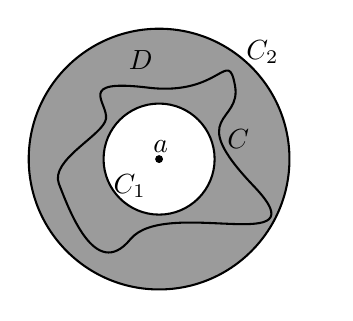
\begin{tikzpicture}[x=0.4,y=0.4,yscale=-1,xscale=1]
%uncomment if require:
\path (0,240.79999542236328);
%set diagram left start at 0, and has height of 240.79999542236328

%Shape: Circle [id:dp6258198346024846] 
\draw  [fill={rgb, 255:red, 155; green, 155; blue, 155 }  ,fill opacity=1 ] (0.77,120.35) .. controls (0.77,55.3) and (53.5,2.57) .. (118.55,2.57) .. controls (183.6,2.57) and (236.32,55.3) .. (236.32,120.35) .. controls (236.32,185.4) and (183.6,238.12) .. (118.55,238.12) .. controls (53.5,238.12) and (0.77,185.4) .. (0.77,120.35) -- cycle ;
%Shape: Circle [id:dp07560041299187703] 
\draw  [fill={rgb, 255:red, 255; green, 255; blue, 255 }  ,fill opacity=1 ] (68.39,120.35) .. controls (68.39,92.65) and (90.85,70.19) .. (118.55,70.19) .. controls (146.25,70.19) and (168.71,92.65) .. (168.71,120.35) .. controls (168.71,148.05) and (146.25,170.51) .. (118.55,170.51) .. controls (90.85,170.51) and (68.39,148.05) .. (68.39,120.35) -- cycle ;
%Shape: Circle [id:dp4185264747557642] 
\draw  [fill={rgb, 255:red, 0; green, 0; blue, 0 }  ,fill opacity=1 ] (116,120.35) .. controls (116,118.94) and (117.14,117.8) .. (118.55,117.8) .. controls (119.96,117.8) and (121.1,118.94) .. (121.1,120.35) .. controls (121.1,121.76) and (119.96,122.9) .. (118.55,122.9) .. controls (117.14,122.9) and (116,121.76) .. (116,120.35) -- cycle ;
%Shape: Polygon Curved [id:ds19792072871438626] 
\draw   (108.6,55.8) .. controls (174.6,63.8) and (180.6,18.8) .. (187.1,53.8) .. controls (193.6,88.8) and (141,78.8) .. (204.1,144.8) .. controls (267.2,210.8) and (124.6,153.8) .. (92.6,192.8) .. controls (60.6,231.8) and (36.72,164.55) .. (28.1,142.8) .. controls (19.47,121.05) and (68.77,98.46) .. (70.6,83.8) .. controls (72.43,69.14) and (42.6,47.8) .. (108.6,55.8) -- cycle ;

% Text Node
\draw (120,108.8) node    {$a$};
% Text Node
\draw (102,30.8) node    {$D$};
% Text Node
\draw (92,144.8) node    {$C_{1}$};
% Text Node
\draw (212,23.8) node    {$C_{2}$};
% Text Node
\draw (190,101.8) node    {$C$};

\end{tikzpicture}

  \caption{単純閉曲線$C$}
\end{wrapfigure}
複素関数$f(z)$が点$a$を孤立特異点に持つとする。
また、点$a$を中心とする円$C_1, C_2$
($C_1$の中に$a$以外の特異点があっても良く、
$C_2$は$C_1$の外側にあるとする)
によって囲まれる領域を$D$とする。
$C_1, C_2$上、領域$D$のいずれにも特異点がないとき、
領域$D$内の任意の$z$に対し、
$D$内にあって$C_1$を囲むような単純閉曲線$C$を使って
\begin{subequations}
\begin{align}
    f(z)
    &= \sum_{n=-\infty}^{\infty}
        c_n (z-a)^n
\label{Laurent series expansion}
\\
    c_n
    &:= \dfrac{1}{2 \pi i}
    \oint_C dz_0 \dfrac{f(z_0)}{(z_0 - a)^{n+1}}
\end{align}
\end{subequations}
が成り立つ。
これを$f(z)$の$a$周りでのLaurent級数展開という。
特に(\ref{Laurent series expansion})の右辺のうち
$c_{-n}\ (n > 0)$が現れる項を特異部(singular part、主要部、principal part)、
$c_{n}\ (n \ge 0)$が現れる項を正則部(regular part、analytic part)という。

\subsubsection{極(pole)、真性特異点(essential singularity)、零点(zero)}

極とは、以下に定める孤立特異点の一種である。
$f(z)$が$a$を$m\ (>0)$位の極($m$-th order pole)
に持つとは、
$f(z)$のLaurent級数展開が$c_{-m} \neq 0$かつ
$n>m$に対し$c_{-n}=0$を満たすことを言う。
特に$1$位の極を単純極(simple pole)、
$2$位の極を二重極(double pole)、
$3$位ならtriple pole、などともいう。

Laurent展開の特異部が有限次で切れず
負べきの項が無限個現れる場合、
$a$を真性特異点(essential singularity)という。

$f(z)$が$a$を$m$位の零点($m$-th order zero)
に持つとは、
$f(z)$のTaylor級数展開
(\ref{Taylor series expansion})
が$c_{m} \neq 0$かつ
$0 \le n < m$に対し$c_{n}=0$を満たすことを言う。
正則関数の零点は孤立し、
この事実を零点孤立の原理という。

\subsubsection{留数定理(Residue theorem)}

Laurent級数展開
\begin{align}
    f(z)
    &= \sum_{n=-\infty}^{\infty}
        c_n (z-a)^n
\end{align}
において、
$\Res{f(z)dz, a} := c_{-1}$を
$f(z)$の点$z=a$における留数(Residue)という。
ただし本来これはRiemann球面$\mathbb{C}P^1$上の
微分形式に対し定義されるものだと示すため、
単に$f(z)$ではなく$f(z)dz$と書いた。
特に、
$f(z)$が$a$を$m$位の極
に持つときは
\begin{align}
    \Res{f(z)dz, a}
    =
    \lim_{z \to a}
    \dfrac{1}{(m-1)!}
    \dfrac{d^{m-1}}{dz^{m-1}}
    \bigg[
        (z-a)^m f(z)
    \bigg]
\end{align}
が成り立つ。
$f(z)$が単純閉曲線$C$内で
$n$個の孤立特異点$a_1,\dots,a_n$を除き正則であるとき
\begin{align}
    \oint_C dz\ f(z)
    =
    2 \pi i \sum_{k=1}^n
    \Res{f(z)dz, a_k}
\end{align}
が成り立つ。

座標変換$u := \dfrac{1}{z}$のもとで
$    g(u)
:=
    f
    \left( \dfrac{1}{u} \right)
$と定義すると、
微分形域は
\begin{align}
    f(z) dz
    =
    f
    \left( \dfrac{1}{u} \right)
    \dfrac{\partial z}{\partial u}
    du
    =
    - \dfrac{ g (u) }{u^2}
    du
\end{align}
のように変換するため、
無限遠点$z = \infty$での留数および
その周りのLaurent展開は
$C_{0}, C_{\infty}$
を原点、無限遠点を囲む
反時計回りの円とし
\begin{subequations}
\begin{align}
    g(u)
&=
    f
    \left( \dfrac{1}{u} \right)
=
    \sum_{n=-\infty}^{\infty}
        c_{n} u^{-n}
=
    \sum_{n=-\infty}^{\infty}
        a_n u^n
\\
    a_n
    &:= \dfrac{1}{2 \pi i}
    \oint_{C_0} du_0 \dfrac{g(u_0)}{u_0^{n+1}}
=
    \dfrac{1}{2 \pi i}
    \oint_{- C_\infty}
        dz_0
        \dfrac{- 1}{z_0^2}
        \dfrac{
            f ( z_0 )
        }{z_0^{-n-1}}
\notag\\&
=
    \dfrac{1}{2 \pi i}
    \oint_{C_\infty}
        dz_0
        \dfrac{
            f ( z_0 )
        }{z_0^{-n+1}}
    = c_{-n}
\\
    \Res{f(z)dz, \infty}
& = c_{-1} =
    \dfrac{1}{2 \pi i}
    \oint_{C_{\infty}} dz\ f(z)
=
    \dfrac{1}{2 \pi i}
    \oint_{- C_{0}} du
    \dfrac{ -1 }{u^2}
    g(u)
=   a_1
\end{align}
\end{subequations}
と書ける。
因子$\dfrac{-1}{u^2}$まで含める事で、
$f(z)$のLaurent展開と$g(z)$のそれが
矛盾なく座標変換で結び付くことが分かる。

\subsubsection{Morera's theorem(モレラの定理)}

以下の意味で、Cauchyの積分定理の逆が成り立つ:
単連結領域$D$で$f(z)$が連続で、
\begin{align}
    \oint_C dz\ f(z) = 0
\end{align}
が$D$内の任意の閉曲線$C$に対し成り立つとする。
このとき$f(z)$は$D$上で正則である。

\newpage
\subsection{初等関数および特殊関数}

\subsubsection{指数関数}

指数関数(exponential function)を
\begin{align}
    \exp(x)
    :=
    \sum_{n=0}^\infty
    \dfrac{x^n}{n!}
\end{align}
により定める。
この級数は複素平面全体で絶対収束
(absolutely convergent)
$\displaystyle
\sum_{n=0}^\infty
\dfrac{|x|^n}{n!}
< \infty
$するため、
$\exp(z)$は整関数
(entire function、複素平面全体で正則な関数)を与える。

\subsubsection{三角関数、双曲線関数}

余弦(cosine)関数、
正弦(sine)関数、
正接(tangent)関数を
指数関数を用いて
\begin{subequations}
\begin{align}
    \cos\theta &:= \dfrac{e^{i\theta} + e^{-i\theta}}{2}
\\
    \sin\theta &:= \dfrac{e^{i\theta} - e^{-i\theta}}{2i}
\\
    \tan\theta &:= \dfrac{\sin\theta}{\cos\theta}
\end{align}
\end{subequations}
と定義する。
これらを総称して三角関数
(trigonometric function、circular function)
という。

同様に双曲線関数(hyperbolic function)を
\begin{subequations}
\begin{align}
    \cosh\theta
    &:=
    \dfrac{e^{\theta} + e^{-\theta}}{2}
    =
    \cos(-i\theta)
\\
    \sinh\theta
    &:=
    \dfrac{e^{\theta} - e^{-\theta}}{2}
    =
    i\sin(-i\theta)
\\
    \tanh\theta
    &:=
    \dfrac{\sinh\theta}{\cosh\theta}
\end{align}
\end{subequations}
と定義する。
それぞれ
hyperbolic cosine、
hyperbolic sine、
hyperbolic tangentと言うが、
$\cosh, \sinh, \tanh$の記号は
cosine hyperbolic(またはコッシュ)、
sine hyperbolic(またはシンチ)、
tangent hyperbolic(またはタンチ)
などと発音される。
native English speakerでも
シンチとかタンチとか言う人は居るが、
分かりづらいだけでなく
はっきり言ってクソダサいので
cosine hyperbolic、sine hyperbolic
などという方が良いと思う。

\subsubsection{無限乗積展開}

三角関数、双曲線関数について
\begin{subequations}
\begin{align}
    \sin \pi x
    &=
    \pi x
    \prod_{n=1}^\infty
    \left(
        1 - \dfrac{x^2}{n^2}
    \right)
\label{infinite product of sine}
\\
    \sinh \pi x
    &=
    \pi x
    \prod_{n=1}^\infty
    \left(
        1 + \dfrac{x^2}{n^2}
    \right)
\label{infinite product of sine hyperbolic}
\\
    \cos \dfrac{\pi x}{2}
    &=
    \prod_{n=1}^\infty
    \left(
        1 - \dfrac{x^2}{(2n-1)^2}
    \right)
\\
    \cosh \dfrac{\pi x}{2}
    &=
    \prod_{n=1}^\infty
    \left(
        1 + \dfrac{x^2}{(2n-1)^2}
    \right)
\end{align}
\end{subequations}
が成り立つ。

\subsubsection{$\Gamma$関数}

$\Gamma$関数は$\Re z > 0$の複素数$z$に対し
\begin{align}
    \Gamma(z)
    := \int_0^\infty dt\ t^{z-1} e^{-t}
\end{align}
により定義され、
その性質
$\Gamma(1) = 1, \Gamma(z+1) = z\Gamma(z)$
から階乗(factorial)
\begin{align}
    \Gamma(n+1) &= n!
    \quad
    (n \in \mathbb{N}_{\ge0})
\end{align}
の複素数への一般化を与える。

重要な応用として、
Gaussian integral(ガウス積分)
\begin{align}
    I :=
    \Gamma\left(\dfrac{1}{2}\right)
    =
    \int_{0}^{\infty} dt\ t^{-1/2}e^{-t}
    =
    2
    \int_{0}^{\infty} dx\ e^{-x^2}
    =
    \int_{-\infty}^{\infty} dx\ e^{-x^2}
    > 0
    \quad(t=x^2)
\end{align}
を求める事を考えよう。
極座標に書き換えると
\begin{align}
    I^2 &=
    \int_{-\infty}^{\infty} dx
    \int_{-\infty}^{\infty} dy
    \ 
        e^{-(x^2 + y^2)}
=
    \int_0^{\infty} dr
    \int_0^{2\pi} r d\theta
    \ 
        e^{-r^2}
\notag\\&=
    2 \pi
    \int_0^{\infty} dr
    \ r 
        e^{-r^2}
=
    \pi
    \int_0^{\infty} dt\ e^{-t}
    \quad(t:=r^2,\ dt = 2 r dr)
\notag\\&=
    \pi\Gamma(1)
    = \pi
\end{align}
すなわち
$\Gamma\left(\dfrac{1}{2}\right)
= I = \sqrt{\pi}$
が求まる。
初等的な置換積分により
\begin{align}
    \int_{-\infty}^{\infty} dx\ e^{-ax^2}
    =
    \sqrt{
        \dfrac{\pi}{a}
    }
\label{gaussian integral}
\end{align}
もすぐ分かり、より一般に
$n \in \mathbb{N}_{\ge0}$に対して
\begin{align}
    \Gamma\left( n + \dfrac{1}{2} \right)
    &=
    \int_0^\infty dt\ t^{n-1/2} e^{-t}
\notag\\&=
    \left[
        \left(
            -
            \dfrac{d}{da}
        \right)^n
        \int_0^\infty dt\ t^{-1/2} e^{-at}
    \right]_{a=1}
\notag\\&=
    \left[
    \left(
        -
        \dfrac{d}{da}
    \right)^n
        a^{-1/2}
        \int_0^\infty a dt\ (at)^{-1/2} e^{-at}
    \right]_{a=1}
\notag\\&=
    \left[
    \left(
        -
        \dfrac{d}{da}
    \right)^n
    \sqrt{
        \dfrac{\pi}{a}
    }
    \right]_{a=1}
\notag\\&=
    \dfrac{(2n-1)!!}{2^{n}}\sqrt{\pi}
\label{Gamma function at half integer}
\end{align}
が得られる。
ただしdouble factorial(二重階乗)を
偶数、奇数それぞれについて
\begin{subequations}
\begin{align}
    (2n)!!
    &:=
    \prod_{i=1}^n (2i)
    =2\cdot4\cdot6\cdots(2n-2)(2n)
\\
    (2n-1)!!
    &:=
    \prod_{i=1}^n (2i-1)
    =
    1\cdot3\cdot5\cdots(2n-3)(2n-1)
\end{align}
\end{subequations}
と定義した。

$\Gamma$関数の$\Re z < 0$への解析接続は
Euler's reflection formula
\begin{align}
    \Gamma(z) \Gamma(1-z)
    =
    \dfrac{\pi}{\sin(\pi z)}
\label{Euler's reflection formula}
\end{align}
で与えられ、
この公式からも
$\Gamma \left(\dfrac{1}{2}\right) = \sqrt{\pi}$
が確かめられる。
$\Gamma$関数は零点を持たないが
(\ref{Euler's reflection formula})からも分かるように
$n \in \mathbb{N}_{\ge0}$に対して
$x = - n$を$1$位の極に持ち、
その周りで
\begin{align}
    \Gamma(x)
    &=
    \dfrac{(-1)^n}{n!}
    \left(
        \dfrac{1}{x+n} - \gamma
        + \sum_{k=1}^n \dfrac{1}{k}
    \right)
    + \mathcal{O}(x+n)
\\
    \gamma
    &:=
    \lim_{n\to\infty}
    \left(
        \sum_{k=1}^n \dfrac{1}{k} 
        -
        \log n
    \right)
    \simeq 0.5772
\end{align}
と展開できる。
ただし$\gamma$は
Euler-Mascheroni constant(オイラー定数)である。

なお、上で与えた$\Gamma$関数の解析接続や
極周りでの展開は
Euler-Mascheroni constantを使って
\begin{subequations}
\begin{align}
    \dfrac{
        e^{- \gamma x}
    }{
        \Gamma(x+1)
    }
    &=
    \prod_{n=1}^\infty
    \left(
        1 + \dfrac{x}{n}
    \right)
    e^{- x / n}
\\
    \dfrac{\sin \pi x}{\pi x}
    &=
    \prod_{n = - \infty}^\infty
    \left(
        1 + \dfrac{x}{n}
    \right)
    e^{- x / n}
\end{align}
\end{subequations}
なる無限乗積展開から正当化される。

\subsubsection{Fresnel integral}

Fresnel integral(フレネル積分)は
Gauss積分
(\ref{gaussian integral})の
$\alpha \in \mathbb{C}$への拡張であり、
\begin{align}
    \int_{-\infty}^{\infty}
    dx\ e^{- \alpha x^2}
    =
    \sqrt{
        \dfrac{\pi}{\alpha}
    }
    \quad
    \text{ for $\Re \alpha \ge 0$}
\label{fresnel integral}
\end{align}
と求まる。

\subsubsection{行列のGauss積分:
    実対称行列の場合}

$N$次元の
実対称行列$A$は
直交行列により対角化可能
\begin{align}
    {}^t O_{ik} A_{kl} O_{lj}
=
    \lambda_i \delta_{ij}
\end{align}
である。
ここで$\lambda_i$は$A$の$i$番目の固有値であって、
右辺の添え字$i$については和を取っていない。
このとき、
$y_i := {}^t O_{ij} x_j
= x_j O_{ji}$
を定義すると
逆変換は
$x_i = ({}^t O)^{-1}_{ij} y_j
= O_{ij} y_j$で与えられ、
\begin{align}
    x_i A_{ij} x_j
&=
    x_i \delta_{ik}
    A_{kl}
    \delta_{ln} x_n
=
    ( x_i O_{ij} )
    ( {}^t O_{jk} A_{kl} O_{lm} )
    ( {}^t O_{mn} x_n )
\notag\\&=
    y_j
    (\lambda_j \delta_{jm})
    y_m
&&
    \text{(カッコ内では$j$について
    和を取らない)}
\notag\\&=
    \lambda_j y_j^2
&&
    \text{($j$について
    一度だけ和を取る)}
\end{align}
のような書き換えが出来る。
行列$A$が正定値
(全ての固有値が正
$\forall i, \lambda_i > 0 $)
であることを仮定すると、
直交行列の性質$\det O = \pm 1$から
変数変換のJacobianが
$J = \det \left(
        \dfrac{\partial x_i}
        {\partial y_j}
    \right)
= \det (O_{ij})
= \pm 1$
となることに気を付けて
Gauss積分の行列への一般化
\begin{align}
    &
    \int_{-\infty}^{\infty}
        \prod_{i=1}^{N}
    \left(
        \frac{dx_i} { \sqrt{2\pi} }
    \right)
    \exp \left(
        - \frac{1}{2}
        x_i A_{ij} x_j
    \right)
=
    \int_{-\infty}^{\infty}
        |J|
    \prod_{i=1}^{N}
    \left(
        \frac{dy_i}{\sqrt{2\pi}}
    \right)
    \exp \left(
        - \frac{1}{2}
        \sum_j
        \lambda_j y_j^2
    \right)
\notag\\&=
    \prod_{i=1}^{N}
    \left[
        \int_{-\infty}^{\infty}
        \frac{dy_i}{ \sqrt{ 2\pi } }
        \exp \left(
            - \frac{\lambda_i}{2}
            y_i^2
        \right)
    \right]
=
    \prod_{i=1}^{N}
    \left[
        \frac{1}{ \sqrt{ 2\pi } }
        \sqrt{
            \dfrac{\pi}{
                \left(
                    \dfrac{\lambda_i}{2}
                \right)
            }
        }
    \right]
=
    \dfrac{1}{
        \sqrt{
            \displaystyle
            \prod_{i=1}^{N} \lambda_i
        }
    }
=
    \frac{1}{
        \sqrt{ \det A }
    }
\label{eq:gaussian-integral-matrix}
\end{align}
が得られる。

なお行列の対角化は一意的でなく、
特に$A$を対角化する行列$O$の
異なる$2$つの列vectorを入れ替えて
$O'$を構成した場合、
$O'$は再び$A$を対角化する
(対角化後の固有値$\lambda_i$の
現れる順番が変化するに過ぎない)。
行列式の反対称性から
$\det( O' ) = - \det( O )$
が成り立つので、
$J = \det( O ) = 1$
に限って議論しても一般性は失わない。

\subsubsection{行列のGauss積分:
    source項のある場合}

次にsource項$\bm{J} \cdot \bm{x} = J_i x_i$
を足して
\begin{align}
    - \frac{1}{2}
    x_i A_{ij} x_j
    + x_i J_i
\end{align}
が指数関数の肩に乗っている場合の
Gauss積分を考えよう。
再び$A$は対称で正定値であることを仮定するので
$\det (A) > 0$すなわち$A$は可逆であり、
$y_i = x_i
    - (A^{-1})_{ij} J_j$
とおくと
\begin{align}
    - \frac{1}{2}
    x_i A_{ij} x_j
    + x_i J_i
&=
    - \frac{1}{2}
    (y_i + (A^{-1})_{ij} J_j)
    A_{ij}
    (y_j + (A^{-1})_{jk} J_k)
+
    (y_i + (A^{-1})_{ij} J_j)
    J_i
\notag\\&=
    - \frac{1}{2}
    (y_i + (A^{-1})_{ij} J_j)
    (A_{ij} y_j + \delta_{ik} J_k)
+
    y_i J_i
+
    J_i (A^{-1})_{ij} J_j
\notag\\&=
    - \frac{1}{2}
    (
        y_i A_{ij} y_j
        + y_i J_i
        + y_j ({}^t A)_{ji}
        (A^{-1})_{il} J_l
        + J_i (A^{-1})_{ij} J_j
    )
    + y_i J_i + J_i
    (A^{-1})_{ij} J_j
\notag\\&=
    - \frac{1}{2}
    \left[
        y_i A_{ij} y_j
        - y_i J_i
        + y_i ({}^t A)_{ij}
        (A^{-1})_{jl} J_l
    \right]
+
    \frac{1}{2} J_i
    (A^{-1})_{ij} J_j
\notag\\&=
    - \frac{1}{2}
    y_i A_{ij} y_j
    +
    \frac{1}{2} J_i
    (A^{-1})_{ij} J_j
\label{eq:variable-convert-with-non-homo-term}
\end{align}
を得る。
ただし、最後の変形では$A$の対称性
$A_{ij} = ({}^t A)_{ij}$より、
$ J_i - ({}^t A)_{ij}
    (A^{-1})_{jl} J_l
= J_i - A_{ij} (A^{-1})_{jl} J_l
= J_i - \delta_{il} J_l 
= J_i - J_i
= 0$
であることを使った。

あとは
(\ref{eq:gaussian-integral-matrix})
の導出と全く同様にして
\begin{align}
    &
    \int_{-\infty}^{\infty}
    \prod_{i=1}^{N}
    \left(
        \frac{dx_i}{ \sqrt{2\pi} }
    \right)
    \exp \left(
        - \frac{1}{2}
        x_i A_{ij} x_j
        + x_i J_i
    \right)
=
    \int_{-\infty}^{\infty}
    \prod_{i=1}^{N}
    \left(
        \frac{dy_i}{ \sqrt{2\pi} }
    \right)
    \exp \left(
        - \frac{1}{2}
        y_i A_{ij} y_j 
        + \frac{1}{2}
        J_i (A^{-1})_{ij} J_j
    \right)
\notag\\&=
    \frac{1}{ \sqrt{\det (A) } }
    \exp\left(
        \frac{1}{2}
        J_i (A^{-1})_{ij} J_j
    \right)
\label{eq:gaussian-integral-with-source}
\end{align}
を得る。
指数関数は複素全平面で解析的なので、
留数定理より
$J_i$を複素変数としても
積分結果は変わらない事に注意しよう。

%参考: http://david-k-zhang.com/notes/gaussian-integrals.html
%4. Multiple Dimensions
% http://www.physik.uzh.ch/~marzocca/QFT2/exercises/Solution01.pdf
% https://terrytao.wordpress.com/2013/02/19/supercommutative-gaussian-integration-and-the-gaussian-unitary-ensemble/

\subsubsection{行列のGauss積分:
    Hermitian行列の場合}

Hermitian行列$A = A^\dagger$は
unitary行列$U$
($U^\dagger = U^{-1}$)により
$U^\dagger_{ij} A_{jk} U_{kl}
= \lambda_i \delta_{il}$
のように対角化できる
(いま$A$はhermitianで正定値なので
$\lambda_i > 0$)ので、
$z_i := U_{ij}^\dagger x_j$
と定義すると
$x_i = U_{ij} z_j$であって
\begin{align}
    &
    - x^*_i A_{ij} x_j
    + x^*_i J_i
    + J^*_i x_i
=
    - (U^*_{ij} z^*_j)
    A_{ik}
    (U_{kl} z_l)
    + (U^*_{ij} z^*_j)
    J_i
    + J^*_i
    (U _{ij} z_j)
\notag\\&=
    - z^*_j
    (U^\dagger_{ji} A_{ik} U_{kl})
    z_l
    + J_i U^*_{ij} z^*_j
    + J^*_i U_{ij} z_j
=
    - z^*_j
    (\lambda_j \delta_{jl})
    z_l
    + J_i (U^\dagger)_{ji} z^*_j
    + J^*_i U_{ij} z_j
\notag\\&
=
    - \lambda_j
    \left(
        z^*_j
        - \frac{ J^*_i U _{ij} }{\lambda_j}
    \right)
    \left(
        z_j
        - \frac{ (U^\dagger)_{jk} J_k }{\lambda_j}
    \right)
    + \frac{
        J^*_i U _{ij}
        (U^\dagger)_{jk} J_k
    }{\lambda_j}
\end{align}
が分かる。
このとき
$z_j
    -
    \dfrac{ (U^\dagger)_{jk} J_k }{\lambda_j}
= x_j + i y_j$
($x_i, y_i \in \mathbb{R}$)
と変数変換すると、
$U^\dagger_{ij} A_{jk} U_{kl} 
= \lambda_i \delta_{il}$
の両辺に左から
$U^\dagger_{pn} (A^{-1})_{nm} U_{mi}$
を掛けて
$\delta_{pl}
= U^\dagger_{pn} (A^{-1})_{nm} U_{ml} \lambda_l$
(ただし右辺の$l$については和を取らない)
すなわち
$\dfrac{\delta_{pl}}{\lambda_l}
= U^\dagger_{pn} (A^{-1})_{nm} U_{ml}$
が得られることに注意して
\begin{align}
    - x^*_i A_{ij} x_j
    + x^*_i J_i
    + J^*_i x_i
&=
    - \lambda_j
    \left( x^2_j + y_j^2 \right)
    + J^*_i U _{ip}
    \frac{ \delta_{pl} }{\lambda_l}
    U^\dagger_{lk} J_k
%\notag\\&
=
    - \lambda_j
    \left( x^2_j + y_j^2 \right)
    + J^*_i (A^{-1})_{ik} J_k
\end{align}
が分かる。

結局、複素平面上の積分測度を
$dz_i d\bar{z}_i := 2 i dx_i dy_i$
と定義
(係数$2 i$は$x_i, y_i$の定義から
Jacobianを計算すると自然に表れる)
すると
(\ref{eq:gaussian-integral-with-source})
の複素積分への自然な拡張
\footnote{
    (\ref{eq:variable-convert-with-non-homo-term})
    の変形は
    任意の可逆な対称行列$A$について成り立つため、
    正定値行列$A$がHermitian行列ではなく
    複素対称行列である場合、
    (\ref{eq:gaussian-integral-with-source})
    のより自然な拡張
    (複素平面への解析接続)が得られる。
    この際、指数関数の解析性から
    積分経路を複素平面上で並進または回転しても
    積分値が変わらない事を用いている。
    なお、複素対称行列(複素共役を含むHermitian行列ではなく)への拡張であることは、
    解析接続が正則関数についてしか定義されないことを反映している。
    式が変数の複素共役を含んでいた場合、このような拡張は可能ではない。
}
として
\begin{align}
    &
    \int_{-\infty}^{\infty}
    \prod_{i=1}^{N}
    \left(
        \frac{dx_i d\bar{x}_i}{2\pi}
    \right)
    \exp \left(
        - x^*_i A_{ij} x_j
        + x_i^* J_i
        + J^*_i x_i
    \right)
\notag\\&=
    \int_{-\infty}^{\infty}
    \prod_{i=1}^{N}
    \left(
        i \frac{dx_i dy_i}{\pi}
    \right)
    \exp \left[
        - \lambda_j
        \left( x^2_j + y_j^2 \right)
        + J^*_i (A^{-1})_{ik} J_k
    \right]
\notag\\&=
    \exp \left(
        J^*_i (A^{-1})_{ik} J_k
    \right)
    \prod_{i=1}^{N}\left[
        \frac{i}{\pi}
    \int_{-\infty}^{\infty}
        dx_i
        \exp \left(
            - \lambda_i
            x^2_i
        \right)
    \int_{-\infty}^{\infty}
        dy_i
        \exp \left(
            - \lambda_i
            y_i^2 
        \right)
    \right]
\notag\\&=
    \exp \left(
        J^*_i (A^{-1})_{ik} J_k
    \right)
    \prod_{i=1}^{N}
    \left[
        \frac{i}{\pi}
        \sqrt{\frac{\pi}{\lambda_i}}
        \sqrt{\frac{\pi}{\lambda_i}}
    \right]
\notag\\&=
    \frac{ i^N }{ \det(A) }
    \exp \left(
        J^*_i (A^{-1})_{ik} J_k
    \right)
\end{align}
が成り立つ。
ただし、$x_j \to z_j$の変数変換ではJacobianは
unitary行列$U$の行列式
(すなわち絶対値$1$の複素数)
となって、
$\bar{x}_j \to \bar{z}_j$から出る
Jacobianと打ち消し合った。
また、$z_j \to (x_j, y_j)$の変数変換では
複素平面の虚軸方向へ積分していることを反映して
Jacobian $2i$が現れるが、
むしろ$y$を純虚に取って
$z = x + y, \bar{z} = x - y$
としておくとこの$i$倍を気にする必要はなくなる。

\subsubsection{超幾何関数
    (hyper-geometric function)
}

Pochhammer symbolを
\begin{align}
    (x)_n
    &:=
    \dfrac{\Gamma(x+n)}{\Gamma(x)}
\end{align}
で定義する。
一般化された超幾何関数
(generalized hyper-geometric function)は
$|z| < 1$で収束するべき級数
\begin{align}
    {}_r F_s
    (
        a_1, \dots, a_r;
        b_1, \dots, a_s;
        z
    )
    &:=
    \sum_{n=0}^{\infty}
    \dfrac{ (a_1)_n \cdots (a_r)_n }{
      (b_1)_n \cdots (b_s)_n
    }
    \dfrac{z^n}{n!}  
\end{align}
で定義される解析関数で、
$a_1, \dots, a_r$同士、
または$b_1, \dots, b_s$同士を交換しても
全く同じ関数を与える。

このうち、特に
\begin{align}
    F(a, b, c; z)
    :=
    {}_2 F_1 (a, b; c; z)
\end{align}
をGaussの超幾何関数、
\begin{align}
    F(a, b; z)
    :=
    {}_1 F_1(a; b; z)
\end{align}
を合流型超幾何関数
(confluent hyper-geometric function)、
あるいは
Kummerの関数などという。

\subsubsection{Sturm-Liouville equation}

任意の$2$階線形微分方程式は
Sturm-Liouville equation
(スツルム・リウビル型微分方程式)
に変形できる。
その解についてはかなり一般論
(離散固有値を持つ、
直交性を満たす、
多くの場合Rodrigues' formula
(ロドリゲス表示、ロドリグ公式など)で書けるなど)
が存在し、
Sturm-Liouville理論と呼ばれる。

\subsubsection{Hermite多項式}
\label{hermite polynomial}

Hermite多項式はHermite微分方程式
\begin{align}
    y'' + x y' + n y = 0
\end{align}
の解であり、
$H_0(x) = 1, H_1(x) = x$として次の漸化式
\begin{subequations}
\begin{align}
    0
    &=
    H_{n+1}(x)
    -
    x H_n(x)
    +
    n H_{n-1}(x)
\\
    H_n'(x)
    &=
    n H_{n-1}(x)
\end{align}
\label{hermite polynomial recurrence relation}
\end{subequations}
および直交性
\begin{align}
    \int dx H_n(x) H_m(x) e^{-x^2/2}
    =
    n! \sqrt{2 \pi}
    \delta_{nm}
\label{normality of hermite polynomial}
\end{align}
を満たす。

Rodrigues' formulaは
\begin{align}
    H_n(x)
    =
    (-1)^n e^{ + x^2 / 2 }
    \dfrac{d^n}{dx^n}
    e^{ - x^2 / 2 }
\label{hermite rodrigues formula}
\end{align}
と与えられ、
合流型超幾何関数$F$を使って
\begin{subequations}
\begin{align}
    H_{2n}(x)
    :=
        (-1)^n
        (2 n - 1)!!
    F(-n, 1/2; x^2/2)
\\
    H_{2n+1}(x)
    :=
        (-1)^n
        (2 n + 1)!!
    F(-n, 3/2; x^2/2)
\end{align}
\end{subequations}
とも書かれる。

\subsubsection{Bessel関数}

第一種Bessel関数
(Bessel function of the first kind)
は一般化された超幾何関数を用い
\begin{subequations}
\begin{align}
    J_\nu (z)
&=
    \dfrac{ (z/2)^\nu }
        { \Gamma(\nu + 1) }
    {}_0 F_1 \left(
        \nu + 1; - \dfrac{z^2}{4}
    \right)
\\&=
    \dfrac{ (z/2)^\nu }
        { \Gamma(\nu + 1) }
    e^{- i z}
    {}_1 F_1 \left(
        \nu + \dfrac{1}{2};
        2 \nu + 1;
        2 i z
    \right)
\end{align}
\end{subequations}
の表示を持つ。
平面波はBessel関数により
\begin{align}
    e^{ i z \sin \theta }
&=
    \sum_{n = - \infty}^{\infty}
        J_n(z)
        e^{i n \theta}
\label{plane wave expanded by bessel 1st}
\end{align}
と展開される。

$\Re \nu > -\dfrac{1}{2},
\Re z > 0$
の領域では
Lommelの積分表示
\begin{align}
    \dfrac{
        \pi^{1/2}
        \Gamma(\nu + \frac{1}{2})
    }
    {(z/2)^\nu}
    J_{\nu}(z)
&=
    \int_{0}^\pi
        d \theta
        \cos (z \cos \theta)
        \sin^{2 \nu} \theta
\label{lommel integral formula for Bessel 1st}
\end{align}
によっても表示できる。

半整数次のBessel関数は初等関数を用い
\begin{align}
    J_{n + 1/2} (z)
&=
    \sqrt{ \dfrac{2}{\pi} }
    z^{n + 1/2}
    \left(
        - \dfrac{1}{z}
        \dfrac{d}{dz}
    \right)^n
    \dfrac{\sin z}{z}
\label{half integral bessel 1st w.r.t. sin}
\end{align}
のように表される。

\newpage
\subsection{Fourier級数展開、Fourier変換}

\subsubsection{Fourier級数展開}

周期$2L$の周期関数$f(x)$、
あるいは区間$(a, a + 2L)$を定義域とする関数$f(x)$を
周期関数に拡張したものについて
\begin{subequations}
\begin{align}
    \tilde{f}(x)
    &:=
    \sum_{n=-\infty}^\infty
    c_n e^{ i\frac{n \pi}{L}x }
\\
    c_n
    &:=
    \dfrac{1}{2L} \int_{-L}^L dx\ 
    f(x) e^{ - i\frac{n \pi}{L}x }
\end{align}
\end{subequations}
を複素Fourier series(フーリエ級数)、
\begin{subequations}
\begin{align}
    \tilde{f}(x)
    &:=
    \dfrac{a_0}{2}
    +
    \sum_{n=1}^\infty
    \left(
        a_n \cos \dfrac{n \pi}{L}x
        +
        b_n \sin \dfrac{n \pi}{L}x
    \right)
\\
    a_n
    &:=
    \dfrac{1}{L} \int_{-L}^L dx\ 
    f(x) \cos\dfrac{n \pi}{L}x
\\
    b_n
    &:=
    \dfrac{1}{L} \int_{-L}^L dx\ 
    f(x) \sin\dfrac{n \pi}{L}x
\end{align}
\end{subequations}
をFourier seriesなどという。
特に$\forall n$に対して
$a_n = 0$のときFourier正弦展開、
$b_n = 0$のときFourier余弦展開
などということもある。

$f(x)$が区分的になめらか、
つまり$f(x), f'(x)$がともに区分的に連続ならば
そのFourier級数は各点収束し、収束先は
\begin{align}
    \tilde{f}(x) = \dfrac{f(x+0) + f(x-0)}{2}
\end{align}
で与えられる。
$f(x)$が連続ならさらに強くFourier級数は関数列として一様収束するが、
不連続関数のFourier級数は一様収束せず、
広義一様収束、ないしコンパクト一様収束
(uniformly convergent on compact sets)
しかしない。
不連続点$x = a$ s.t.
$\mathrm{Disc}(f,a) := f(a+0) - f(a-0) \neq 0$の付近では
振幅$\mathrm{Disc}(f,a) \times 0.08949\dots$程度の振動が起こり、
ギブス現象(Gibbs phenomenon)とか呼ばれる。
激しく振動する成分はRiemann-Lebesgue lemmaより積分に寄与しないので、
$L^2$-normで見る限り(\ref{convergence of norm})と全く同様に
\begin{subequations}
\begin{align}
    \lim_{N\to\infty}\bigg|\bigg|
        f(x) - \tilde{f}_N(x)
    \bigg|\bigg|^2
    &=
    \lim_{N\to\infty}\int dx
    \Big| f(x) - \tilde{f}_N(x) \Big|^2
    = 0
\\
    \tilde{f}_N(x)
    &:=
    \sum_{n=-N}^N
    c_n e^{ i\frac{n \pi}{L}x }
\end{align}
\end{subequations}
のように収束している、ということである。

\subsubsection{Fourier変換}

周期関数でないより一般の関数もFourier級数と同様に
三角関数で展開したいというのは自然な要求だろう。
特にこれは微分方程式を解くために役立つ。
急減少関数$f(x)$のFourier transform(フーリエ変換)$\tilde{f}(k)$
および
inverse Fourier transform(逆フーリエ変換)を
\begin{subequations}
\begin{align}
    \tilde{f}(k)
    &:=
    \int dx\ f(x) e^{-ikx}
\\
    f(x)
    &=
    \dfrac{1}{2\pi}\int dk\ 
    \tilde{f}(k) e^{+ikx}
\end{align}
\label{fourier transf}
\end{subequations}
で定める。
特に、逆変換はDirac delta関数のFourier表示
(\ref{dirac delta fourier representation})
により正当化される。
$\dfrac{1}{2\pi}$を
Fourier変換(逆変換でなく)の定義に付けて
$\displaystyle
\tilde{f}(k) = \dfrac{1}{2\pi}
\int dx\ f(x) e^{-ikx}$
としたり、
$k$の符号を逆にして
$\displaystyle
\tilde{f}(k) =
\int dx\ f(x) e^{+ikx}$としたり、
(\ref{plain wave in qm})のように
波動関数の規格化を気にする量子力学では
$\displaystyle
    \braket{ x | f }
    =
    \dfrac{1}{\sqrt{2\pi}}
    \int dk\ \braket{k | f} e^{+ikx}
    ,
    \braket{ k | f }
    =
    \dfrac{1}{\sqrt{2\pi}}
    \int dx\ \braket{x | f} e^{-ikx}
$
のように$\dfrac{1}{\sqrt{2\pi}}$が
変換と逆変換の両方に現れたり、
数値計算や結晶学では角周波数でなく周波数を用いて
$\displaystyle
\tilde{f}(k) =
\int dx\ f(x) e^{+2\pi ikx}$としたり、
とにかく無数の流儀があるが、本質積な違いは何もない。

Fourier変換は不確定性関係という良くない性質を持つため、
画像処理などの分野ではwavelet解析という拡張を考えることがある。

\newpage
\subsection{微分幾何学}

\subsubsection{計量}

計量(metric tensor)
$g_{ij} = g_{ji}$は対称tensorで、
その逆行列を$g^{ij} := (g^{-1})^{ij}$
(すなわち
$g_{ik} g^{kj} = \delta_i^j$)、
行列式を$g = \det (g_{ij})$と書く。
計量の成分を示すときは行列で書くか、
$ds^2 = g_{ij} dx^i dx^j$の全ての項を
書き下す。
特に、後者の記法では
非対角項($i \neq j$)に対して
対称性から必ず
計量の成分$g_{ij}$の$2$倍
が現れる事に注意しよう。
例えば二次元直交座標を用いて
$z = x + i y,
\overline{z} = x - i y$
と定義される座標での計量は
\begin{subequations}
\begin{align}
    (g_{ij})
&=
    \begin{pmatrix}
        0 & \dfrac{1}{2}
    \\
        \dfrac{1}{2} & 0
    \end{pmatrix}
\notag\\
    (g^{ij})
&=
    \begin{pmatrix}
        0 & 2
    \\
        2 & 0
    \end{pmatrix}
\\
    g
&=
    \det(g_{ij})
    = - \dfrac{1}{4}
\\
    ds^2
&=
    dx^2 + dy^2
=
    d z
    d \overline{z}
=
    g_{z \overline{z}}
    d z
    d \overline{z}
+
    g_{\overline{z} z}
    d \overline{z}
    d z
\neq \dfrac{1}{2} 
    d z
    d \overline{z}
\end{align}
\end{subequations}
となる。

座標$x^i$における
計量$g_{ij}$が与えられているとき、
$\partial_i = \dfrac{\partial}{\partial x^i}$として
scalar関数$f(x)$に作用するLaplacianは
\begin{align}
    \Delta f(x)
    =
    \dfrac{1}{ \sqrt {g} }
    \partial_i
    \left(
        g^{ij}
        \sqrt{ g }
        \partial_j
        f (x)
    \right)
\label{laplacian of scalar in terms of metric}
\end{align}
と書くことが出来る。
ただし
vectorやtensorに作用するLaplacianは
このように書くことが出来ないので注意せよ。

\subsubsection{$n$次元極座標}

$1$次元極座標は
(連続な角度変数が取れないため特殊で)
$(r, \mathrm{sgn}(x)) = (|x|, \pm 1)$
で、
$2$次元極座標は
$(x, y) = (r \cos \theta, r \sin \theta)$
で、
$3$次元球座標は
$(x, y, z)
=
    (r \sin \theta \sin \phi,
    r \sin \theta \cos \phi,
    r \cos \theta)$
で与えられる。

一般の$n (\ge 3)$次元の極座標
(polar coordinates、
球座標、spherical coordinates)
$(r, \theta_1, \theta_2,
\dots, \theta_{n-1})$
は直交座標
$(x_1, \dots, x_n)$を用いて
\begin{subequations}
\begin{align}
    r :=& \sqrt{
        \sum_{i=1}^n
        (x_i)^2
    }
&
    (0 \le\ &r < \infty)
\\
    x_n
    =:&\ 
    r \cos \theta_1
&
    (0 \le\ &\theta_1 \le \pi)
\\
    x_{n-1}
    =:&\ 
    r \cos \theta_2
    \sin \theta_1
&
    (0 \le\ &\theta_2 \le \pi)
\\\notag
    &
    \vdots
    &
    \vdots
\\
    x_{n-i}
    =:&\ 
    r
    \cos \theta_{i+1}
    \prod_{j=1}^{i}
    \sin \theta_j
&
    (0 \le\ &\theta_{i+1} \le \pi)
\\\notag
    &
    \vdots
    &
    \vdots
\\
    x_{2}
    =:&\ 
    r
    \cos \theta_{n-1}
    \prod_{j=1}^{n-2}
    \sin \theta_j
&
    (0 \le\ &\theta_{n-1} < 2 \pi)
\\
    x_{1}
    =:&\ 
    r
    \prod_{j=1}^{n-1}
    \sin \theta_j
\end{align}
\label{n dimensional spherical coordinates}
\end{subequations}
と定義される。
ただし、
$1 \le i \le n-2$に対して
$x_{n-i+1}$の表式に
$\cos \theta_i$が$1$回だけ現れるため、
この因子が左辺の符号を決める
(つまり$\sin \theta_i$が正の値しか取れない)よう
$\theta_i$の取り得る範囲を選んだ。
こうしておけば
$(x_1, \dots, x_n)$と
$(r, \theta_1, \dots, \theta_{n-1})$
が一対一で対応するためである。
$i = n - 1$の時だけが特殊で、
$x_1, x_2$が任意の実数を動くためには
$\cos \theta_{n-1}$だけでなく
$\sin \theta_{n-1}$も正負の値を動けなければならない事に注意せよ。
特に、
$\dfrac
    { x_{1} }
    { x_{2} }
=
    \tan \theta_{n-1}
$
及び
$
\dfrac
    { x_{n - i} }
    { x_{n - (i - 1)} }
=
    \tan \theta_{i}
    \cos \theta_{i+1}
$
$(1 \le i \le n - 2)$
が成り立つ。

明らかに
\begin{subequations}
\begin{align}
    \dfrac{\partial x_i}
        {\partial r}
&=
    \begin{cases}
    \displaystyle
        \prod_{j=1}^{n - 1}
        \sin \theta_j
    &(i = 1)
    \\
    \displaystyle
        \cos \theta_{n - i + 1}
        \prod_{j=1}^{n - i}
        \sin \theta_j
    &(2 \le i \le n - 1)
    \\
    \displaystyle
        \cos \theta_{1}
    &(i = n)
    \end{cases}
\\
    \dfrac{\partial x_i}
        {\partial \theta_j}
&=
    \begin{cases}
    \displaystyle
        r \cos \theta_j
        \prod_{k=1 (\neq j)}^{n-1}
        \sin \theta_k
    &(i = 1 \le j \le n - 1)
    \\
    \displaystyle
        r \cos \theta_{n - i + 1}
        \cos \theta_j
        \prod_{k=1 (\neq j)}^{n - i}
        \sin \theta_k
    &(2 \le i \le n - j \le n - 1)
    \\
    \displaystyle
        -
        r \sin \theta_{n - i + 1}
        \prod_{k=1}^{n - i}
        \sin \theta_k
    &(2 \le i = n - j + 1 \le n - 1)
    \\
    \displaystyle
        0
    &(2 \le n-j+1 \le i - 1 < i \le n - 1)
    \\
    \displaystyle
        -
        r \sin \theta_1
    &(1 = j < i = n)
    \\
    \displaystyle
        0
    &(1 < j < i = n)
    \end{cases}
\end{align}
\end{subequations}
が分かる。
この座標での計量は
\begin{align}
    &
    ds^2
=
    g_{ij} dx^i dx^j
:=
    \delta_{ab}
    \dfrac{\partial x^a}{\partial \phi^i}
    \dfrac{\partial x^b}{\partial \phi^j}
    d \phi^i d\phi^j
\notag\\&
=
    d r^2
\underset{
\displaystyle
\color{blue}
    =
    \Bigg(
    \underset{
    \displaystyle
    = \sin^2 \theta_1
    }{\underline{
        \prod_{j=1}^{n - 1}
        \sin^2 \theta_j
    +
    \sum_{i = 2}^{n-1}
        \cos^2 \theta_{i}
        \prod_{j=1}^{i - 1}
        \sin^2 \theta_j
    }}
    +
        \cos^2 \theta_{1}
    \Bigg)
    = 1
}{\underline{
    \left(
        \prod_{j=1}^{n - 1}
        \sin^2 \theta_j
    +
    \sum_{i = 2}^{n-1}
        \cos^2 \theta_{n - i + 1}
        \prod_{j=1}^{n - i}
        \sin^2 \theta_j
    +
        \cos^2 \theta_{1}
    \right)
}}
\notag\\&\qquad
    +
    (dr d\theta_1 + d\theta_1 dr)
\underset{
\displaystyle
\color{blue}
    =
    r \sin \theta_1
    \cos \theta_1
    \Bigg(
    \underset{
    \displaystyle
        \text{$dr^2$の項と同様に計算すると$1$}
    }{\underline{
        \prod_{q=2}^{n-1}
        \sin^2 \theta_q
    +
    \sum_{i = 2}^{n - 1}
        \cos^2 \theta_{i}
        r \cos \theta_1
        \prod_{q=2}^{i-1}
        \sin^2 \theta_q
    }}
    -
        1
    \Bigg)
    = 0
}{\underline{
    \Bigg(
        \prod_{p=1}^{n - 1}
        \sin \theta_p
        r \cos \theta_1
        \prod_{q=2}^{n-1}
        \sin \theta_q
    +
    \sum_{i = 2}^{n - 1}
        \cos^2 \theta_{n - i + 1}
        \prod_{p=1}^{n - i}
        \sin \theta_p
        r \cos \theta_1
        \prod_{q=2}^{n - i}
        \sin \theta_q
    -
        \cos \theta_1
        r \sin \theta_1
    \Bigg)
}}
\notag\\&\qquad
    +
    \sum_{k=2}^{n-1}
    (dr d\theta_k + d\theta_k dr)
    \Bigg(
\underline{
        \prod_{p=1}^{n - 1}
        \sin \theta_p
        r \cos \theta_k
        \prod_{q=1 (\neq k)}^{n-1}
        \sin \theta_q
    +
    \sum_{i = 2}^{n-k}
        \cos^2 \theta_{n - i + 1}
        \prod_{p=1}^{n - i}
        \sin \theta_p
        r
        \cos \theta_k
        \prod_{q=1 (\neq k)}^{n - i(\ge k)}
        \sin \theta_q
}
\notag\\&\qquad\qquad
\underset{
\displaystyle
\color{blue}
    =
    r \tan^{-1} \theta_k
    \bigg(
    \underbrace{
        \prod_{p=1}^{n - 1}
        \sin^2 \theta_p
    +
    \sum_{i = k+1}^{n - 1}
        \cos^2 \theta_{i}
        \prod_{p=1}^{i - 1}
        \sin^2 \theta_p
    }_{\substack{
    \displaystyle
    = \sin^2 \theta_1
        -
        \sum_{i = 2}^k
        \cos^2 \theta_{i}
        \prod_{p=1}^{i - 1}
        \sin^2 \theta_p
    \\
    \displaystyle
    =
        \sin^2 \theta_1
        -
        \bigg(
            \sin^2 \theta_1
        -
            \prod_{p=1}^{k}
            \sin^2 \theta_p
        \bigg)
    }}
    -
    \underbrace{
        \sin^2 \theta_k
        \prod_{p=1}^{k - 1}
        \sin^2 \theta_p
    }_{\substack{
    \displaystyle
        =
        \prod_{p=1}^{k}
        \sin^2 \theta_p
    }}
    \bigg)
    = 0
}{\underline{
    -
        \cos \theta_{k}
        \prod_{p=1}^{k - 1}
        \sin \theta_p
        r
        \sin \theta_{k}
        \prod_{q=1}^{k - 1}
        \sin \theta_q
    \Bigg)
}}
\notag\\&\qquad
    + d \theta_1^2
    \bigg\{
\underbrace{
        r^2 \cos^2 \theta_{1}
        \prod_{p=2}^{n-1}
        \sin^2 \theta_p
    +
    \sum_{i = 2}^{n-1}
        r^2 \cos^2 \theta_{n - i + 1}
        \cos^2 \theta_1
        \prod_{p=2}^{n-i}
        \sin^2 \theta_p
}_{\substack{
    \displaystyle
    \color{blue}\text{
    $dr d\theta_1$の項と同様に
    $r^2 \cos^2 \theta_1$
}}}
    +
        r^2 \sin^2 \theta_1
    \bigg\}
\notag\\&\qquad
    +
    \sum_{k = 2}^{n - 2}
    d \theta_k^2
\underbrace{
    \Bigg\{
        r^2 \cos^2 \theta_k
        \prod_{p=1 (\neq k)}^{n-1}
        \sin^2 \theta_p
    +
    \sum_{i = 2}^{n - k}
        r^2 \cos^2 \theta_{n - i + 1}
        \cos^2 \theta_{k}
        \prod_{p=1 (\neq k)}^{n-i(\ge k)}
        \sin^2 \theta_p
}_{\substack{
\displaystyle
\color{blue}
    = r^2 \tan^{-2} \theta_k
    \Bigg(
\underbrace{
        \prod_{p=1}^{n-1}
        \sin^2 \theta_p
    +
    \sum_{i = k+1}^{n - 1}
        \cos^2 \theta_{i}
        \prod_{p=1}^{i-1}
        \sin^2 \theta_p
}_{\substack{
\displaystyle
\color{blue}
    \text{
        $dr d\theta_k$の項と同様に
        $\displaystyle
        \prod_{p=1}^{k}
        \sin^2 \theta_p
        $
    }
}}
    \Bigg)
    = r^2 \cos^2 \theta_k
    \prod_{p=1}^{k-1}
    \sin^2 \theta_p
\\
}}
% \notag\\&\qquad\qquad
    +
\underbrace{
        r^2 \sin^2 \theta_{k}
        \prod_{p=1}^{k-1}
        \sin^2 \theta_p
}_{\substack{
\displaystyle
\color{blue}
    =
    r^2 \bigg(
        \prod_{p=1}^{k}
        \sin^2 \theta_p
    \bigg)
}}
    \Bigg\}
\notag\\&\qquad
    + d \theta_{n-1}^2
    \bigg\{
        r^2 \cos^2 \theta_{n-1}
        \prod_{p=1}^{n-2}
        \sin^2 \theta_p
    +
        r^2 \sin^2 \theta_{n-1}
        \prod_{p=1}^{n-2}
        \sin^2 \theta_p
    \bigg\}
    -
\underbrace{
    \sum_{k = 1}^{n - 1}
    \sum_{l \neq k}
    d \theta_k
    d \theta_l
}_{\substack{
\displaystyle
\color{blue} =
    2
    \sum_{l < k}
    d \theta_k
    d \theta_l
%\\ \displaystyle \color{blue}
=
    2 \sum_{k = 2}^{n - 1}
    \sum_{l = 1}^{k-1}
    d \theta_k
    d \theta_l
}}
    \underbrace{
    \bigg\{
        \cdots
    \bigg\}
    }_{\substack{\displaystyle
        \color{blue} = 0
    }}
\notag\\&
=
    d r^2
+
    r^2
\left(
        d \theta_1^2
    +
    \sum_{k=2}^{n-1}
        d\theta_k^2
    \prod_{p=1}^{k-1}
        \sin^2 \theta_p
\right)
\label{n dim spherical coord metric}
\end{align}
と計算できる
($l \neq k$の項が消えることを確かめてみよ)。
特に、$g_{ij}$が対角なことから
\begin{align}
    g =
    \det ( g_{ij} )
=
    1 \cdot (r^2)^{n-1}
    \prod_{k=2}^{n-1}
    \prod_{p=1}^{k-1}
        \sin^2 \theta_p
=
    r^{2(n-1)}
    \prod_{j = 1}^{n-2}
    \sin^{2(n - j - 1)} \theta_j
\end{align}
がすぐに分かる。

$n (\ge 3)$次元における体積要素は
Jacobian
\begin{align}
    \frac{\partial(x_1, x_2, \cdots, x_n)}
    {\partial(r, \theta_1, \cdots, \theta_{n-1})}
=
    \det
\left(
    \dfrac{\partial x_i}{\partial \phi_j}
\right)
=
    \sqrt{ g }
=
    r^{n-1}
    \prod_{j = 1}^{n-2}
    \sin^{n - j - 1} \theta_j
\label{jacobian for spherical coordinates}
\end{align}
に気を付けて
\begin{align}
    d^n x
&=
    \prod_{i = 1}^n
    d x_i
=
    \frac{\partial(x_1, x_2, \cdots, x_n)}
    {\partial(r, \theta_1, \cdots, \theta_{n-1})}
    \prod_{i = 1}^n
    d \phi_i
=
    d r d \theta_1
        \cdots d \theta_{n-1}
    r^{n-1}
    \prod_{j = 1}^{n-2}
    \sin^{n - j - 1} \theta_j
\\\notag&
\bigg(
=
    (dr)
    (r d \theta_1)
    (r \sin \theta_1 d \theta_2)
\cdots
    (r \prod_{j = 1}^i
    \sin \theta_j d \theta_i)
\cdots
    (r \prod_{j = 1}^n
    \sin \theta_j d \theta_n)
\bigg)
\end{align}
で与えられ、
特に半径$R$の$n$次元球の体積は
\begin{align}
    V_n(R)
&:=
    \int_{r \le R} d^n x
=
    \int_0^R
        dr
    \int_0^{2 \pi}
        d \theta_{n-1}
    \prod_{i=1}^{n-2}
    \left[
        \int_0^{\pi}
            d \theta_i
    \right]
    r^{n-1}
    \prod_{j = 1}^{n-2}
    \sin^{n - j - 1} \theta_j
\notag\\&
=
    \int_0^R
        dr\ 
    r^{n-1}
    \int_0^{2 \pi}
        d \theta_{n-1}
    \prod_{i=1}^{n-2}
    \left[
        \int_0^{\pi}
            d \theta_i
        \sin^{n - i - 1} \theta_i
    \right]
\notag\\&
=
    \dfrac{R^n}{n}
    2 \pi
    \prod_{i=1}^{n-2}
    \left[
        \sqrt{\pi}
        \dfrac{\Gamma(\frac{n - i}{2})}
        {\Gamma(\frac{n - i + 1}{2})}
    \right]
\notag\\&
=
    \dfrac{R^n}{n}
    S_{n-1}
\end{align}
と求まる。
ここで$S_{n-1}$は$n-1$次元
単位球面$S^{n-1}$の面積で、
対応する立体角を$d^{n-1} \Omega$
と書くことにすると
$\Gamma$関数の半整数での値
(\ref{Gamma function at half integer})
を用いて
\begin{align}
    S_{n-1}
&=
    \int_{r = 1}
        d^{n-1} \Omega
=
    2 \pi
    \prod_{i=1}^{n-2}
    \left[
        \sqrt{\pi}
        \dfrac{\Gamma(\frac{n - i}{2})}
        {\Gamma(\frac{n - i + 1}{2})}
    \right]
=
    2 \pi
    \pi^{(n-2)/2}
    \dfrac{
        \cancel{
            \Gamma(\frac{n - 1}{2})
        }
    }
        {\Gamma(\frac{n}{2})}
    \dfrac{
        \cancel{
            \Gamma(\frac{n - 2}{2})
        }
    }
        {\cancel{
            \Gamma(\frac{n - 1}{2})
        }}
    \cdots
    \dfrac{\Gamma(\frac{n - (n-2)}{2})}
        {\cancel{
            \Gamma(\frac{n - (n-2) + 1}{2})
        }}
\notag\\&
=
    2
    \pi^{n/2}
    \dfrac{\Gamma(1)}
        {\Gamma(\frac{n}{2})}
=
    \dfrac{ 2 \pi^{n/2} }
        {\Gamma(\frac{n}{2})}
\label{surface area of n dimensional sphere}
\end{align}
と書ける。

公式(\ref{laplacian of scalar in terms of metric})
に
計量
(\ref{n dim spherical coord metric})
および
Jacobian
(\ref{jacobian for spherical coordinates})
を代入すると、
$n$次元球座標でscalarに作用する
Laplacianは
\begin{align}
    \Delta f(x)
&=
    \dfrac{1}{ \sqrt {g} }
    \partial_i
    \left(
        g^{ij}
        \sqrt{ g }
        \partial_j
        f (x)
    \right)
\notag\\&
=
    \dfrac{1}{
    \displaystyle
        r^{n-1}
        \prod_{p = 1}^{n-2}
        \sin^{n - p - 1} \theta_p
    }
    \partial_i
    \left(
        g^{ij}
        r^{n-1}
        \prod_{q = 1}^{n-2}
        \sin^{n - q - 1} \theta_q
        \partial_j
        f (x)
    \right)
\notag\\&
=
    \dfrac{1}{
    \displaystyle
        r^{n-1}
    }
    \partial_r
    \left(
        r^{n-1}
        \partial_r
        f
    \right)
+
    \dfrac{1}{
    \displaystyle
        \sin^{n - 2} \theta_1
    }
    \partial_1
    \left(
        r^{-2}
        \sin^{n - 2} \theta_1
        \partial_1
        f
    \right)
\notag\\&\qquad
+
\sum_{k = 2}^{n-2}
    \dfrac{1}{
    \displaystyle
        \sin^{n - k - 1} \theta_k
    }
    \partial_k
    \left(
    \left[
        r^{-2}
        \prod_{p=1}^{k-1}
        \sin^{-2} \theta_p
    \right]
        \sin^{n - k - 1} \theta_k
        \partial_k
        f
    \right)
\notag\\&\qquad
+
    \partial_{n-1}
    \left(
        \left[
            r^{-2}
            \prod_{p=1}^{n-2}
            \sin^{-2} \theta_p
        \right]
        \partial_{n-1}
        f
    \right)
\notag\\&
=
    \dfrac{1}{
    \displaystyle
        r^{n-1}
    }
    \partial_r
    \left(
        r^{n-1}
        \partial_r
        f
    \right)
+
    \dfrac{1}{r^2}
        \Delta_{S^{n-1}}
        f
\label{n dim laplacian in polar coordinates}
\end{align}
と書けることが分かる。
第$1$項は
$    \dfrac{1}{
    \displaystyle
        r^{n-1}
    }
    \partial_r
    \left(
        r^{n-1}
        \partial_r
    \right)
=
    \partial_r^2
    +
    \dfrac{n-1}{ r }
        \partial_r
$と書いても同じことである。
ただし、角度方向つまり
球面$S^{n-1}$上のLaplace-Beltrami operator
(ラプラス・ベルトラミ作用素)を
\begin{align}
    \Delta_{S^{n-1}} f
&:=
        \dfrac{1}{
    \displaystyle
        \sin^{n - 2} \theta_1
    }
    \partial_1
    \left(
        \sin^{n - 2} \theta_1
        \partial_1
        f
    \right)
+
\sum_{k = 2}^{n-2}
    \dfrac{1}{
    \displaystyle
        \sin^{n - k - 1} \theta_k
        \prod_{p=1}^{k-1}
        \sin^{2} \theta_p
    }
    \partial_k
    \left(
        \sin^{n - k - 1} \theta_k
        \partial_k
        f
    \right)
\notag\\&\qquad
+
    \dfrac{1}{
    \displaystyle
        \prod_{p=1}^{n-2}
        \sin^{2} \theta_p
    }
    \partial_{n-1}^2
        f
\notag\\&
=
    \sum_{k = 1}^{n - 1}
    \prod_{p = 1}^{k}
    \dfrac{1}{\sin^2 \theta_p}
    \dfrac{1}{\sin^{n - k - 3} \theta_k}
    \partial_k
    \left(
        \sin^{n - k - 1} \theta_k
        \partial_k
        f
    \right)
\label{spherical Laplacian}
\end{align}
と定義した。
この微分作用素は球Laplacian
(spherical Laplacian)と呼ばれる事もあり、
物理の文脈では
角運動量の大きさoperator
(\ref{the square of the magnitude of the orbital angular momentum})
の$\bm{x}$-表示に他ならない。
$\Delta_{S^{n-1}}$の固有関数を
球面調和関数と呼ぶが、
これも$\hat{L}^2$の固有状態
$\ket{j, m}$に対応する波動関数と解釈できる。
なお、この結果は$n = 2,3$で
\begin{align}
    \Delta_{(2)}
    &=
    \dfrac{1}{r}
        \partial_r
        (r \partial_r)
    +
    \dfrac{1}{r^2}
    \Delta_{S^1}
\notag\\&
=
    \dfrac{1}{r}
        r \partial_r^2
    +
    \dfrac{1}{r}
        \partial_r
    +
    \dfrac{1}{r^2}
    \dfrac{1}{\sin^2 \theta}
    \dfrac{1}{\sin^{2-1-3} \theta}
    \partial_\theta
    (\sin^{2-1-1} \theta \partial_\theta)
\notag\\&
=
        \partial_r^2
    +
        \dfrac{1}{r}
        \partial_r
    +
    \dfrac{1}{r^2}
    \partial_\theta^2
\\
    \Delta_{(3)}
    &=
    \dfrac{1}{r^2}
        \partial_r
        (r^2 \partial_r)
    +
    \dfrac{1}{r^2}
    \Delta_{S^2}
\notag\\&
=
    \partial_r^2
    +
    \dfrac{2}{r}
        \partial_r
    +
    \dfrac{1}{r^2}
    \left[
        \dfrac{1}{\sin^2 \theta}
        \dfrac{1}{\sin^{3-1-3} \theta}
        \partial_\theta
        \left(
            \sin^{3-1-1} \theta
            \partial_\theta
        \right)
    +
        \dfrac{1}{\sin^2 \theta}
        \dfrac{1}{\sin^2 \phi}
        \dfrac{1}{\sin^{3-2-3} \phi}
        \partial_\phi
        \left(
            \sin^{3-2-1} \phi
            \partial_\phi
        \right)
    \right]
\notag\\&
=
    \partial_r^2
    +
    \dfrac{2}{r}
        \partial_r
    +
    \dfrac{1}{r^2}
    \left[
        \dfrac{1}{\sin \theta}
        \partial_\theta
        \left(
            \sin \theta
            \partial_\theta
        \right)
    +
        \dfrac{1}{\sin^2 \theta}
        \partial_\phi^2
    \right]
\end{align}
のように知られた結果を再現する。

\subsubsection{微分形式}

\newpage
\subsection{Dirac DeltaとGreen関数}

\subsubsection{Diracの$\delta$関数}

$f(x)$はなめらかで$|x| \to \infty$で十分早く
$0$に収束する関数
(急減少ないし緩増加関数、より一般には
コンパクト台(compact support)を持つ関数)
であるとする。
このように適当なよい性質を持つ関数を
試行関数(test function)と言い、
任意の試行関数$f(x)$に対して
\begin{align}
    \int dx f(x) \delta(x - a)
    =
    f(a)
\end{align}
を満たす$\delta$を
Diracのdelta関数(Dirac delta function)
という。
特に、$a$を含まない任意の区間で$\delta(x - a)$を
積分しても$0$になってしまう。

明らかに、普通の実関数は上のような性質を満たすことは出来ない。
Diracのdeltaは超関数
(Schwartz distributionまたはgeneralized function)
として定式化され、
あるいは佐藤超関数(hyperfunction)として
$x = x_0$で正則な関数に対し
Plemeljの公式
\begin{align}
    \delta(x - x_0)
:=
    \pm
    \dfrac{1}{\pi}
    \Im
    \dfrac{1}{x - x_0 \mp i \epsilon}
=
    \pm
    \dfrac{1}{2 \pi i}
    \left[
        \dfrac{1}{x - x_0 \mp i \epsilon}
        -
        \dfrac{1}{x - x_0 \pm i \epsilon}
    \right]
\end{align}
により定式化することもできる。
$x = x_0$で正則な関数$f(x)$について
$f(x) \delta(x - x_0)$の実軸上での積分は
\begin{align}
    \int dx
    f(x) \delta(x - x_0)
&=
    \pm
    \int
    \dfrac{dx}{2 \pi i}
    f(x)
    \left[
        \dfrac{1}{x - x_0 \mp i \epsilon}
        -
        \dfrac{1}{x - x_0 \pm i \epsilon}
    \right]
\notag\\&
=
    \pm
    \dfrac{1}{2 \pi i}
    \left[
    \int_{- \infty \mp i \epsilon}
        ^{+ \infty \mp i \epsilon}
        dx
    -
    \int_{- \infty \pm i \epsilon}
        ^{+ \infty \pm i \epsilon}
        dx
    \right]
    \dfrac{f(x)}{x - x_0}
\notag\\&
=
    \dfrac{1}{2 \pi i}
    \oint_{\text{around } x_0}
        dx
    \dfrac{f(x)}{x - x_0}
\notag\\&
=
    f(x_0)
\end{align}
とDirac Delta関数の定義を満たすことが確かめられる。
特に係数の$\pm$は
$\oint dx$が$x_0$の周りを
反時計まわりに回るよう定義されている事により
吸収された。

Dirac delta関数のFourier表示は
\begin{align}
    \delta(x-y)
    =
    \int
    \dfrac{dk}{2\pi}
    e^{ik(x-y)}
\label{dirac delta fourier representation}
\end{align}
のように与えられる。

Dirac deltaの微分は部分積分によって定義される。
すなわち、
$\dfrac{d \delta}{dx}
    (x - x_0)$は
任意の滑らかな関数$f(x)$に対し
\begin{align}
    \int dx
    f(x)
    \dfrac{d \delta}{dx}
    (x - x_0)
=
    -
    \int dx
    \dfrac{d f(x)}{dx}
    \delta(x - x_0)
=
    -
    \dfrac{d f(x_0)}{dx}
\label{derivative of delta function}
\end{align}
を与える関数である。

\subsubsection{Green関数の定義}

適当な線形微分operator $D(x)$を考える。
ただし、微分operatorが線形(linear)であるとは
その関数$f(x)$への作用が
$f(x)$によらず決まるという意味であり、
作用が$x$に依っていてもよい。
あるいはoperator $\hat{O}$
(の$\bm{x}$-表示)が
関数$\psi_1(x) = \braket{x | \psi_1},
\psi_2(x) = \braket{x | \psi_2}$
に作用して
(\ref{linearity of an operator})
の意味で線形性を持つと言っても
同じことである。
例として$\dfrac{d}{dx} + \sin x$や
$\exp( i a \dfrac{d}{dx}) + x^3$
などは線形operatorであり、
$D f(x) = \left(
    \dfrac{d f}{dx}
\right)^2$
すなわち$D[f] = \dfrac{d f}{dx}
    \dfrac{d}{dx}$
は線形operatorではない。

与えられた線形operator $D(x)$に対し、
適当な境界条件及び
\begin{align}
    D(x) G(x, x')
    =
    \delta(x - x')
\end{align}
を満たす関数$G(x, x')$を$D(x)$の
グリーン関数(Green's function)と言う。
適当な関数$f(x)$について
$g(x)$を与えられた関数として
$D(x) f(x) = g(x)$
という形の微分方程式に名前が付いている場合には、
その方程式のGreen関数という言い方をする場合もある。
数学の微分方程式論の分野では
方程式の全ての項を左辺に寄せて書く
古い流儀があった名残として
\begin{align*}
    D(x) G(x, x')
    +
    \delta(x - x')
&=
    0
\\\therefore
    D(x) G(x, x')
&=
    -
    \delta(x - x')
\end{align*}
のように符号違いで$G$を定義する事もあるが、
本質的な違いはない。
もし$G(x, x')$が求まれば、
非斉次項付きの線形微分方程式
\begin{align}
    D(x) f(x)
    =
    \rho(x)
\end{align}
の($G$に対応する境界条件のもとでの)
解は
\begin{align}
    f(x) =
    \int dx'\ 
        G(x, x')
        \rho(x')
\label{convolution representation of green function solution}
\end{align}
と書ける事が直接の計算
\begin{align}
    D(x) f(x)
&=
    \int dx'\ 
        \rho(x')
    D(x)
        G(x, x')
=
    \int dx'\ 
        \rho(x')
    \delta (x - x')
=
    \rho(x)
\end{align}
から確かめられる。

\subsubsection{階段関数}

ヘヴィサイドの階段関数(Heaviside step function)は
\begin{align}
    \theta(x)
    :=
    \begin{cases}
        1 & (x > 0)
    \\
        0 & (x < 0)
    \end{cases}
\label{definition of step function}
\end{align}
と定義される。
明らかに
\begin{subequations}
\begin{align}
    \theta(- x) &= 1 - \theta(x)
\\
    \mathrm{sgn}(x)
    &=
    2 \theta(x) - 1
\label{step function and sign}
\end{align}
\end{subequations}
が成り立つ。
階段関数のFourier変換は
正の無限小量$\epsilon$を使って
\begin{align}
  \theta(t)
  &=
    - \int\dfrac{d \omega'}{2 \pi i}
    \dfrac{e^{- i \omega' t}}{\omega' + i \epsilon}
\label{fourier transformation of step function}
\end{align}
と書け、
その著しい性質として
微分がDirac delta
(\ref{dirac delta fourier representation})
となること
\begin{align}
    \left(
        \dfrac{d}{dt}
        +
        \epsilon
    \right)
    \theta(t)
=
    - \int\dfrac{d \omega'}{2 \pi i}
    \dfrac{
        - i \omega' + \epsilon
    }{\omega' + i \epsilon}
    e^{- i \omega' t}
=
    - \int\dfrac{d \omega'}{2 \pi i}
    e^{- i \omega' t}
    ( - i)
=
    \delta(x)
\label{derivative of step function}
\end{align}
が挙げられる。
すなわち、$\theta(t)$は
微分operator $\dfrac{d}{dt}$の
Green関数になっている。

\subsubsection{$n$次元LaplacianのGreen関数}

$n$次元Laplacian
(Laplace operator、Laplace演算子)
\begin{align}
    \Delta_{(n)}
    :=
    \sum_{i=1}^n
    \left(
        \dfrac{\partial}{\partial x^i}
    \right)^2
    =
    \partial_i^2
\end{align}
のGreen関数を求めよう。
これにより、
関数$f(x)$についての
Poisson方程式(Poisson's equation)
\begin{align}
    \Delta_{(n)} f(x)
    &= g(x)
\label{poisson eq}
\end{align}
(ただし$g(x)$は与えられた関数)
の適当な境界条件の下での解が
積分
(\ref{convolution representation of green function solution})
によって得られる。
典型的には、静的な場合のMaxwell方程式
(\ref{static eq for ele-mag scalar potential})
がこの形をしている。

また、Laplace方程式(Laplace's equation)
\begin{align}
    \Delta_{(n)} f(x)
    &= 0
\label{laplace eq}
\end{align}
はPoisson方程式の特別な場合であり、
この方程式を満足する$f(x)$を
調和関数という。

$1$次元の場合、
\begin{align}
    \dfrac{d}{dx}
    |x - x_0|
=
    \mathrm{sgn}
    (x - x_0)
\end{align}
に気が付けば、
階段関数の性質
(\ref{step function and sign})
及びその微分
(\ref{derivative of step function})
から
\begin{subequations}
\begin{align}
    &
    \Delta_{(1)}
    |x - x_0|
=
    \dfrac{d^2}{dx^2}
    |x - x_0|
=
    \dfrac{d}{dx}
    \mathrm{sgn}
    (x - x_0)
=
    \dfrac{d}{dx}
    2 \theta (x - x_0)
=
    2 \delta (x - x_0)
\\\therefore
&\qquad
    \Delta_{(1)}
    \dfrac{1}{2}|x - x_0|
    =
    \delta (x - x_0)
\end{align}
\end{subequations}
が得られる。

$2$次元の場合は極座標
$r := \sqrt{x^2 + y^2}$
を使うと話が簡単で、
$n$次元では
$\displaystyle
\delta_{ii}
= \sum_{i=1}^n 1
= n$
が成り立つことに気を付けると、
$r \neq 0$では明らかに
\begin{subequations}
\begin{align}
    \partial_i
    \log r
&=
    \dfrac{x_i}{r}
    \dfrac{1}{r}
=
    \dfrac{x_i}{r^2}
\\
    \Delta_{(2)}
    \log r
&=
    \partial_i^2
    \log r
=
    \partial_i
    \dfrac{x_i}{r^2}
=
    \dfrac{
        \delta_{ii} r^2
    -
        x_i (2 r)
        \dfrac{x_i}{r}
    }{r^4}
=
    \dfrac{
        2 r^2
    -
        r^2 (2 r)
        \dfrac{1}{r}
    }{r^4}
= 0
\end{align}
\end{subequations}
が成り立つ。
ただし原点$r = 0$では振る舞いが特異的で、
半径$r = R$の円の外向き
面素vector(と言っているが、
今の場合円周$S^1$に垂直な
$1$次元vector)が
$dS = R d \theta$
すなわち
\begin{align}
    d \bm{S}
=
    \left(
        \dfrac{x}{R}
    ,
        \dfrac{y}{R}
    \right)
    R d \theta
\end{align}
となることに気を付けて
Gaussの定理を使うと
\begin{align}
    \int d^2 x\ 
        \Delta_{(2)}
        \log r
&=
    \lim_{R \to \infty}
    \oint_{r = R} d \bm{S}
        \cdot
        \nabla
        \log r
=
    \lim_{R \to \infty}
    \oint_{r = R}
        d \theta
    R
    \left[
        \dfrac{x}{R}
        \dfrac{x}{R^2}
    +
        \dfrac{y}{R}
        \dfrac{y}{R^2}
    \right]
\notag\\&
=
    \lim_{R \to \infty}
    \oint
        d \theta
=
    2 \pi
\end{align}
が得られるので、
求めるGreen関数
\begin{align}
    \Delta_{(2)}
    \dfrac{1}{2 \pi}
    \log \sqrt{x^2 + y^2}
=
    \delta(x)
    \delta(y)
=
    \delta(\bm{x})
\end{align}
を得る。

一般次元$n \neq 2$でのGreen関数
$G^{(n)}(\bm{x})$は、
$\delta(\bm{x})$が$r$にしか依らないため
Laplacian
(\ref{n dim laplacian in polar coordinates})
の作用が簡単になり、
$\bm{x} \neq 0$で
\begin{align}
    \Delta_{(n)}
    G^{(n)}(\bm{x})
=
    \dfrac{1}{r^{n-1}}
    \dfrac{\partial}{\partial r}
    \left(
        r^{n-1}
        \dfrac{\partial}{\partial r}
        G^{(n)}(\bm{x})
    \right)
= 0
\end{align}
となる事に気付けば容易に求まる。
上式は簡単に積分出来て
\begin{align}
    &r^{n-1}
    \dfrac{\partial}{\partial r}
    G^{(n)}(\bm{x})
=
    - C
\notag\\
    &G^{(n)}(\bm{x})
=
    \dfrac{C}{(n - 2) r^{n-2}}
    + D
\label{n dim green func of laplace (const unfixed)}
\end{align}
を得る。
最後に無限遠での境界条件
$\lim_{r \to \infty}
    G^{(n)}(\bm{x}) = 0$
及び
全空間での積分の規格化から
定数を決定すると
\begin{align}
    \int d^n x\ 
    \Delta_{(n)}
    G^{(n)}(\bm{x})
=
    \int d \bm{S}
        \cdot
        \nabla
    G^{(n)}(\bm{x})
=
    \int d^{n-1} \Omega\ 
        r^{n-1}
        \dfrac{d}{dr}
    G^{(n)}(\bm{x})
=
    - C S_{n-1}
=    1
\end{align}
から$n$次元球の表面積
(\ref{surface area of n dimensional sphere})
を用い
$C = - \dfrac{1}{S_{n-1}}, D = 0$
を得る。
結局、求めるLaplacianのGreen関数は
\begin{align}
    G^{(n)}(\bm{x})
=
    \begin{cases}
        \dfrac{1}{2}|x|
    &(n = 1)
    \\
    \\
        \dfrac{1}{2 \pi}
        \log \sqrt{x^2 + y^2}    
    &(n = 2)
    \\
    \\
        -
        \dfrac{1}{
            (n - 2) S_{n-1} r^{n-2}
        }
    &(n \ge 3)
    \end{cases}
\label{green function of n dim laplacian}
\end{align}
となる。
特に、$n = 1$では$S_0 = 2$なので
$n \ge 3$の場合と同じ公式を用いて表せる。

\subsubsection{次元正則化}

さて、$n = 2$と$n \neq 2$で
LaplacianのGreen関数
$G^{(n)}(\bm{x})$の
振る舞いが大きく異なることについて
考えてみよう。
その1つの理由は、
低次元$(n = 1,2)$では無限遠で
Green関数が十分早く減衰していない事にある。
境界条件が異なるため、
Green関数の振る舞いも異なるのである。
もう1つの考察として、
次元正則化
(dimensional regularization)
を行ってみよう。
上の表式の
$n = 2 + \epsilon$
への解析接続を考えた後、
$\epsilon \to 0$の極限を取るのである。
すると
\begin{align}
    G^{(2)}_{\rm reg}(\bm{x})
&:=
    \lim_{\epsilon \to 0}
    G^{(2 + \epsilon)}(\bm{x})
=
    -
    \lim_{\epsilon \to 0}
    \dfrac{1}{
        \epsilon
        S_{2 + \epsilon}
    }
    r^{- \epsilon}
=
    -
    \lim_{\epsilon \to 0}
    \dfrac{1}{
        \epsilon
        S_{2 + \epsilon}
    }
    (1 - \epsilon \log r)
=
    -
    \lim_{\epsilon \to 0}
    \dfrac{1}{
        S_{2 + \epsilon}
    }
    \left(
        \dfrac{1}{\epsilon}
    -
        \log r
    \right)
\notag\\&=
    \dfrac{1}{
        2 \pi
    }
        \log r
    + (\text{const.})
=
    G^{(2)}(\bm{x})
    + (\text{const.})
\end{align}
と、無限大に発散する定数項を除いて
正しいGreen関数が得られることが分かる。
定数は無限大であろうとも
微分には効かないので無視する事にする
(あるいは、$n = 1, 2$では
$\lim_{r \to \infty}
    G^{(n)}(\bm{x}) = 0$
なる境界条件は
(\ref{n dim green func of laplace (const unfixed)})
において積分定数$D$を
どのように取っても満たせないため、
$D = 0$の代わりに
$D = \dfrac{1}
    {\epsilon S_{2 + \epsilon}}
    +
    (\text{finite part})$
と取り発散を打ち消したと思っても良い)
と、
$n \ge 3$の場合の表式は
実は任意の次元で成り立っているのである。

更に注意深く、上の議論では
定数$D$のうち
極限$\epsilon \to \infty$
で発散する部分は
$G^{(2)}_{\rm reg}(\bm{x})$
が有限であれという条件から定まったが、
$(\text{finite part})$
と書いた有限部分は
決まらなかった事に意識を向けてみよう。
上では特に気にせず
\begin{align}
    G^{(2)} (\bm{x})
    =
    \dfrac{1}{
        2 \pi
    }
        \log r
\end{align}
と書いていたが、
$\log$の引数は
無次元量でなければならないのであった。
実際には$r$という量は長さの次元を持っており、
同じく長さを持つ適当な定数$a$を使って
$\log (r/a)$としなければならない。
この$a$は境界条件だけからは決まらず、
$(\text{finite part})$
はこの$\log a$の任意性を表している。
実際
(\ref{n dim green func of laplace (const unfixed)})
をよく見ると、
$r
\dfrac{\partial}{\partial r}
G^{(2)}(\bm{x})
=
- C$
という式を積分する際に
\begin{align}
    &G^{(2)}(\bm{x})
    =
        - C
        \int_{a}^r dr
        \dfrac{1}{r}
    =
        - C
        \log (r/a)
\end{align}
というように積分区間の選び方から
自然に定数$a$の自由度が生じることが分かる。
ここで$a \to 0$とすると
積分は発散してしまう
(それ以前の問題として、
$r = 0$付近では
微分方程式
(\ref{n dim green func of laplace (const unfixed)})
の右辺にDirac deltaが現れ、
解も上の形では書けなくなってしまう)
ため、
$a$は考えている物理系のscaleよりも十分
短距離(つまり高energy領域)の物理を
あえて無視するために導入された
UV regulatorであることが分かる。

一般に発散する積分を正則化した際には
このような有限定数の任意性が残り、
理論だけからこれを決めることは出来ない。
実験値との比較により
これを決定する条件のことを
繰り込み条件と呼ぶ。

\subsection{Helmholtz方程式のGreen関数}

Laplace方程式
(\ref{laplace eq})
の一般化である
Helmholtz方程式(Helmholtz equation)
\begin{align}
    (\Delta_{(n)} + k^2)
    f(x)
&= 0
\end{align}
を考えよう。
典型的にはLorenz gauge
\begin{align}
0 =
    \mu_0 \epsilon_0
    \frac{\partial \phi (t, \bm{x})}
      {\partial t}
  +
    \nabla \cdot
      \bm{A} (t, \bm{x})
\end{align}
のもとでのMaxwell方程式
(\ref{maxwell eq of potentials})
を時間についてFourier変換すると
Helmholtz型の微分方程式に帰着する。
あるいは調和振動子の運動方程式
(\ref{newton harm osci eom})
も$1$次元Helmholtz方程式と見做すことが出来る。

なお、今の場合
$A = x_i,
B = \dfrac{d}{dx_i}$
と置くことで
\begin{align}
    \left[
        x_i,
        \dfrac{d}{dx_j}
    \right]
&=
    - \delta_{ij}
\end{align}
が成り立つので、
operatorの固有値を変化する公式
(\ref{finite translation of operator})
により
$\bm{k}^2 = k^2$となる任意のvector
$\bm{k}$を用いて
\begin{align}
    &
    \Delta_{(n)} + k^2
=
    \sum_{i = 1}^n
    \left[
        \dfrac{d^2}{dx_i^2}
    +
        k_i^2
    \right]
=
    \sum_{i = 1}^n
    \left[
    \left(
        \dfrac{d}{dx_i}
    +
        i k_i
    \right)
    \left(
        \dfrac{d}{dx_i}
    -
        i k_i
    \right)
    \right]
\notag\\&
=
    \sum_{i = 1}^n
    \left[
    \left(
        e^{- i \bm{k} \cdot \bm{x}}
        \dfrac{d}{d x_i}
        e^{i \bm{k} \cdot \bm{x}}
    \right)
    \left(
        e^{i \bm{k} \cdot \bm{x}}
        \dfrac{d}{d x_i}
        e^{- i \bm{k} \cdot \bm{x}}
    \right)
    \right]
\end{align}
と書き換えることが出来る。

このGreen関数はもちろん
Laplacianの場合と同様に
Fourier変換と留数定理を用いて求まり、
\begin{align}
    0
&=
    (\Delta_{(n)} + k^2)
    G^{(n)}( \bm{x}, k )
    -
    \delta( \bm{x} )
\notag\\&
=
    (\Delta_{(n)} + k^2)
    \int d^n p\ 
        e^{i \bm{p} \cdot \bm{x}}
        G^{(n)}( \bm{p}, k )
    -
    \int d^n p\ 
        e^{i \bm{p} \cdot \bm{x}}
\notag\\&
=
    \int d^n p\ 
        e^{i \bm{p} \cdot \bm{x}}
    \left[
        (- \bm{p}^2 + k^2)
        G^{(n)}( \bm{p}, k )
    - 1
    \right]
\notag\\\therefore\quad
    G^{(n)}( \bm{p}, k )
&=
    \dfrac{- 1}{\bm{p}^2 - k^2}
\notag\\\Rightarrow\quad
    G^{(n)}( \bm{x}, k )
&=
    \int d^n p\ 
        e^{i \bm{p} \cdot \bm{x}}
        G^{(n)}( \bm{p}, k )
=
    \int d^n p\ 
        e^{i \bm{p} \cdot \bm{x}}
        \dfrac{- 1}{\bm{p}^2 - k^2}
\notag\\&
=
    \int d p\ 
    d^{n-1} \Omega
        \dfrac{
            - p^{n-1}
            e^{i p x \cos \theta_1}
        }{p^2 - k^2}
\end{align}
となる。
最後に積分を極座標表示に直したが、
$p_n$軸を$\bm{x}$の方向に取ったので
$\bm{p} \cdot \bm{x} = px \cos \theta_1$となった。
$i = 2, \cdots, n-1$に対して
$\theta_i$角度積分は
(\ref{surface area of n dimensional sphere})
と同様に実行でき$\displaystyle
2 \pi
\prod_{i=2}^{n-2}
\left[
    \sqrt{\pi}
    \dfrac{\Gamma(\frac{n - i}{2})}
    {\Gamma(\frac{n - i + 1}{2})}
\right]
=
2 \pi^{n/2}
    \dfrac{ \Gamma(1) }{ \Gamma(\frac{n-1}{2}) }
$を出す。
$\theta_1$積分も
Lommelの積分表示
(\ref{lommel integral formula for Bessel 1st})
により第一種Bessel関数に書き換えられて
\begin{align}
    \int_0^\pi d \theta_1
        \sin^{n-2} \theta_i
        e^{i p x \cos \theta_1}
&=
    \dfrac{
        \pi^{1/2}
        \Gamma(
            (\frac{n-2}{2})
            + \frac{1}{2}
        )
    } { (px/2)^{ \frac{n-2}{2} } }
    J_{ \frac{n-2}{2} } (px)
=
    \dfrac{
        \pi^{1/2}
        \Gamma(
            \frac{n-1}{2}
        )
    } { (px/2)^{ \frac{n}{2} - 1 } }
    J_{ \frac{n}{2} - 1 } (px)
\end{align}
を得る。

最後に動径方向の$p$積分は
$t = p x$と置き換えて
\begin{align}
    G^{(n)}( \bm{x}, k )
&=
    \int_0^\infty d p
        \dfrac{
            - p^{n-1}
        }{(p + k)(p - k)}
    2 \pi^{n/2}
        \dfrac{ \Gamma(1) }
            { \Gamma(\frac{n-1}{2}) }
    \dfrac{
        \pi^{1/2}
        \Gamma(
            \frac{n-1}{2}
        )
    } { (px/2)^{ \frac{n}{2} - 1 } }
    J_{ \frac{n}{2} - 1 } (px)
\notag\\&
=
    2 \pi^{(n+1)/2}
    \left(
        \dfrac{2}{x}
    \right)^{ \frac{n}{2} - 1 }
    \int_0^\infty d p
        \dfrac{
            - p^{n/2}
            J_{ \frac{n}{2} - 1 } (px)
        }{(p + k)(p - k)}
\notag\\&
=
    \dfrac{ \pi^{(n+1)/2} }{ k }
    \left(
        \dfrac{2}{x}
    \right)^{ \frac{n}{2} - 1 }
    \int_0^\infty d p\ 
        p^{n/2}
        J_{ \frac{n}{2} - 1 } (px)
    \left[
        \dfrac{ 1 }{p + k}
    -
        \dfrac{ 1 }{p - k}
    \right]
\notag\\&
=
    \dfrac{ \pi^{(n+1)/2} }{ k }
        \dfrac{2^{ n/2 - 1 }}{ x^{n-1} }
    \int_0^\infty d t\ 
        t^{ \frac{n}{2} }
        J_{ \frac{n}{2} - 1 } (t)
    \left[
        \dfrac{ 1 }{t + k x}
    -
        \dfrac{ 1 }{t - k x}
    \right]
\notag\\&
=
    \dfrac{ \pi^{(n+1)/2} }{ k }
        \dfrac{2^{ n/2 - 1 }}{ x^{n-1} }
    \left[
    -
    \int_{- \infty}^0 d t\ 
        t^{ \frac{n}{2} }
        J_{ \frac{n}{2} - 1 } (t)
        \dfrac{
            (-1)^{\frac{n}{2} + \frac{n}{2} - 1 }
        }{t - k x}
    -
    \int_0^\infty d t\ 
        t^{ \frac{n}{2} }
        J_{ \frac{n}{2} - 1 } (t)
        \dfrac{ 1 }{t - k x}
    \right]
\end{align}
となる。
$n =: 2m + 1$が奇数の場合にはこれは
\begin{align}
    G^{(2m+1)}( \bm{x}, k )
&=
    \dfrac{ \pi^{m+1} }{ k }
        \dfrac{2^{ m - 1/2 }}{ x^{2m} }
    \int_{- \infty}^\infty d t\ 
        t^{ m + \frac{1}{2} }
        J_{ m - \frac{1}{2} } (t)
        \dfrac{ - 1
        }{ t - (k x \pm i \epsilon) }
\end{align}
のようにまとめられ
(ただし積分経路上の極を避けるため
分母に無限小の虚部を導入した)、
留数定理および
半整数次のBessel関数の性質
(\ref{half integral bessel 1st w.r.t. sin})
から
\begin{align}
    G^{(2m+1)}( \bm{x}, k )
&=
    - \dfrac{ \pi^{m+1} }{ k }
        \dfrac{2^{ m - 1/2 }}{ x^{2m} }
    (k x)^{ m + \frac{1}{2} }
    J_{ m - \frac{1}{2} } (k x)
\notag\\&
=
    - \dfrac{ \pi^{m+1} }{ k }
        \dfrac{2^{ m - 1/2 }}{ x^{2m} }
    (k x)^{ m + \frac{1}{2} }
    \sqrt{ \dfrac{2}{\pi} }
    (k x)^{(m-1) + 1/2}
    \left(
        - \dfrac{1}{kx^2}
        \dfrac{d}{dk}
    \right)^{m-1}
    \dfrac{\sin (k x)}{ k x }
\notag\\&
=
    - \dfrac{ \pi^{m + 1/2} }{ k }
        \dfrac{
            2^{ m }
            k^{ 2 m }
        }{ x^{2 m - 2} }
    \left(
        - \dfrac{1}{k}
        \dfrac{d}{dk}
    \right)^{m-1}
    \dfrac{\sin (k x)}{ k x }
\end{align}
と導かれる
(でいいのかしら、境界条件とかちゃんとやってないけど
$3$次元$m = 1$では内向き・外向き球面波が出るはずだが
$\dfrac{ 2 \pi^{3/2} \sin (kx) }{x}$
となって$1$次元っぽい見た目になっている)。

\newpage
\section{量子力学の公式}

記号が煩雑になるのを避けるため、
以下では誤解の恐れがない場合は
適宜operatorを表す$\hat{}$を省略する。

\subsection{Operatorの基本的な性質}

\subsubsection{交換関係・反交換関係}

定義$[\hat{A}, \hat{B}]
:= \hat{A}\hat{B} - \hat{B}\hat{A}$
(\ref{commutator definition})
および$\{\hat{A}, \hat{B}\} :=
\hat{A}\hat{B} + \hat{B}\hat{A}$
(\ref{anticommutator definition})
から容易に示される。
証明は読者の演習問題とする。
\begin{align}
    [\hat{A}, \hat{B}] &= - [\hat{B}, \hat{A}]
\\
    \{\hat{A}, \hat{B}\} &= \{\hat{B}, \hat{A}\}
\\
    [\hat{A}, \hat{B}\hat{C}]
   &=
   \hat{B}[\hat{A}, \hat{C}]
+
    [\hat{A}, \hat{B}] \hat{C}
\label{A,BC to B(A,C) + (A,B)C}
\\
    [\hat{A}\hat{B}, \hat{C}]
   &=
   \hat{A}\{\hat{B}, \hat{C}\}
-
    \{\hat{A}, \hat{C}\} \hat{B}
\\
    \{ \hat{A}\hat{B}, \hat{C} \}
   &=
   \hat{A}\{\hat{B}, \hat{C}\}
-
    [ \hat{A}, \hat{C} ] \hat{B}
%\notag\\&
=
   \hat{A} [ \hat{B}, \hat{C} ]
+
    \{\hat{A}, \hat{C}\} \hat{B}
\\
    \left(\hat{A}\hat{B}\right)^\dagger
    &=
    \hat{B}^\dagger\hat{A}^\dagger
\\
    [\hat{A}, \hat{B}]^\dagger
    &=
    [\hat{B}^\dagger, \hat{A}^\dagger]
\end{align}
特に(\ref{A,BC to B(A,C) + (A,B)C})は
繰り返し使うことにより
\begin{align}
    [\hat{A}, \hat{B}_1\hat{B}_2\cdots\hat{B}_n]
   &=
   \sum_{i=1}^n
   \hat{B}_1\cdots\hat{B}_{i-1}
   [\hat{A}, \hat{B}_i]
   \hat{B}_{i+1}\cdots\hat{B}_n
\end{align}
と拡張できる。

\subsubsection{Baker-Campbell-Hausdrff formula}

Baker-Campbell-Hausdrff formulaは
\begin{align}
    e^{\hat{A}} e^{\hat{B}}
    &=
    \exp\left(
        \hat{A} + \hat{B}
        + \dfrac{1}{2}[\hat{A},\hat{B}]
        + \dfrac{1}{12}[\hat{A} - \hat{B},[\hat{A},\hat{B}]]
        + \cdots
    \right)
\label{BCH formula}
\end{align}
である。
証明のためには
$e^{\hat{C}(t)}
= e^{t\hat{A}} e^{t\hat{B}}$
すなわち$\hat{C}(t) = \log (
    e^{t\hat{A}} e^{t\hat{B}}
)$とおき、
右辺のTaylor展開を好きな次数まで計算した後
$t=1$とおけばよい
(類似の証明として
\ref{proof for unitary transf formula for operator}
も参照のこと)。
$t$の次数とoperatorの次数は明らかに一致するので、
次数に応じて交換子の数が増えることも明らかであろう。
特に交換関係が$c$-数
$[\hat{A},\hat{B}]=c$の場合は
交換子を$2$回以上取ると必ず消えるため
\begin{align}
    e^{\hat{A}} e^{\hat{B}}
&=
    \exp\left(
        \hat{A} + \hat{B}
        + \dfrac{1}{2}c
    \right)
\label{simpler BCH formula}
\end{align}
となる。

\subsubsection{Trotter公式}

Lie-Trotter product formula(Trotter公式)は
上のBCH公式(\ref{BCH formula})の自明な系として
\begin{align}
    e^{\hat{A} + \hat{B}}
= \lim_{M \to \infty}
    \left(
        e^{\hat{A}/M} e^{\hat{B}/M}
    \right)^M
\end{align}
の形で与えられ、$M$をTrotter数(Trotter number)という。
証明も上と同様に、
$\hat{C}(t)
= \log( e^{t\hat{A}} e^{t\hat{B}} )
= t \log( e^{t\hat{A}} e^{t\hat{B}} )^{ 1/t }$
で$M := \dfrac{1}{t} \to \infty$
の極限を取ればよい。
\ref{proof for unitary transf formula for operator}
で見るように
Taylor展開の各べきを比較して
(\ref{BCH formula})が得られるのだから、
$t \to 0$の極限でその最低次である
交換子を持たない項のみが残るのは当然である。

\subsection{Unitary Transformation of an Operator}

(\ref{BCH formula})を示すのと全く同様の論法で、
Hermitianとは限らない任意のoperator $A, B$に対して
\begin{align}
    e^A B e^{-A}
    &=
    B + [A,B] + \dfrac{1}{2!}[A,[A,B]]
    +
    \dfrac{1}{3!}[A,[A,[A,B]]]
    +
    \cdots
\label{unitary transf formula for operator}
\end{align}
が示せるが、ここでは一応証明を載せておこう。

\subsubsection{Taylor展開を用いた証明}
\label{proof for unitary transf formula for operator}

記号$C_i$を漸化式
\begin{align}
    \mathrm{C}_0(A,B)
    :=
    B
,\qquad
    \mathrm{C}_{n+1}(A,B)
    :=
    [A,\mathrm{C}_{n}(A,B)]
\end{align}
で定義すると、示すべき式
(\ref{unitary transf formula for operator})は
\begin{align}
    e^{A} B e^{-A}
    &=
    \sum_{n=0}^\infty
    \dfrac{1}{n!}
    \mathrm{C}_{n}(A,B)
\label{rewrite of unitary transf of operator}
\end{align}
となる。
これを示すために実parameter $s$を導入し、
左辺を$s=0$の周りで展開する:
\begin{subequations}
\begin{align}
    e^{sA} B e^{-sA}
    &=
    e^{sA} \mathrm{C}_{0}(A,B)e^{-sA}
\\
    \dfrac{d}{ds}\bigg[
        e^{sA} B e^{-sA}
    \bigg]
    &=
    Ae^{sA} B e^{-sA}
    -
    e^{sA} B A e^{-sA}
    =
    e^{sA} [A,B]e^{-sA}
    =
    e^{sA} \mathrm{C}_{1}(A,B) e^{-sA}
\end{align}
\end{subequations}
ここで$k \ge 0$について
\begin{align}
    \dfrac{d^k}{ds^k}\bigg[
        e^{sA} B e^{-sA}
    \bigg]
    =
    e^{sA} \mathrm{C}_{k}(A,B) e^{-sA}
\end{align}
を仮定すると
\begin{align}
    \dfrac{d^{k+1}}{ds^{k+1}}
    \bigg[
        e^{sA} B e^{-sA}
    \bigg]
&=
    \dfrac{d}{ds}\bigg[
        e^{sA} \mathrm{C}_{k}(A,B) e^{-sA}
    \bigg]
\notag\\&=
    A e^{sA} \mathrm{C}_{k}(A,B) e^{-sA}
    -
    e^{sA} \mathrm{C}_{k}(A,B) Ae^{-sA}
\notag\\&=
    e^{sA} [A,\mathrm{C}_{k}(A,B)] e^{-sA}
\notag\\&=
    e^{sA}  \mathrm{C}_{k+1}(A,B) e^{-sA}
\end{align}
を得るため、帰納法から任意の$n$について
\begin{align}
    \dfrac{d^n}{ds^n}\bigg[
        e^{sA} B e^{-sA}
    \bigg]
    =
    e^{sA} \mathrm{C}_{n}(A,B) e^{-sA}
\end{align}
が示された。
これにより、左辺の$s=0$周りのTaylor級数を得る:
\begin{align}
    e^{sA} B e^{-sA}
&=
    \sum_{n=0}^\infty
        \dfrac{1}{n!}
    \bigg[
        \dfrac{d^n}{ds'^n}
        \bigg(
            e^{s'A} B e^{-s'A}
        \bigg)
    \bigg]_{s'=0}
    s^n
\notag\\&=
    \sum_{n=0}^\infty
        \dfrac{1}{n!}
    \bigg[
        \mathrm{C}_{n}(A,B)
    \bigg]
    s^n
\notag\\&=
    \sum_{n=0}^\infty
        \dfrac{s^n}{n!}
    \mathrm{C}_{n}(A,B)
\end{align}
最後に$s=1$と置けば
\footnote{
与えられた$A, B$に対し、
この級数展開の収束半径が$1$より大きいことは仮定する。
もともとoperatorの関数はTaylor展開
(\ref{function of operator})
で定義されていたので、
Taylor展開出来ない場合を考える必要はない。
}、
左辺の展開が右辺に一致したことになり、
望む公式
(\ref{rewrite of unitary transf of operator})
を得る。

\subsubsection{特殊な場合}

公式
(\ref{unitary transf formula for operator})
において
特に交換関係が$c$-数の場合$[\hat{A}, \hat{B}] = c$には
\begin{align}
    e^{ \hat{A} } \hat{B} e^{ - \hat{A} }
    &=
    \hat{B} + c
\label{finite translation of operator}
\end{align}
が得られ、
operatorの固有値の原点をずらす操作になっていることが分かる。
また、(\ref{unitary operator})の直下で指摘したように
Hermitian operator $\hat{O} = \hat{O}^\dagger$を使って
$\hat{A} = i \hat{O}$と取った場合は
$ e^{ \hat{A} } \hat{B} e^{ - \hat{A} } $
は$\hat{B}$のunitary transformationとなっている。

以上の2つの事実を合わせると、
例えば正準変数
$[\hat{q}_i, \hat{p}_j] = i\hbar\delta_{ij}$
について$\hat{A} = - \dfrac{a}{i\hbar} \hat{p}_j,
\hat{B} = \hat{q}_i$
として公式を使うことで
\begin{align}
    e^{ - \frac{a}{i\hbar} \hat{p}_j }
        \hat{q}_i
    e^{ \frac{a}{i\hbar} \hat{p}_i }
    &=
    \hat{q}_i + a \delta_{ij}
\end{align}
が言える。
これは運動量が並進対称性に対応する保存量であることを反映しており、
より一般の対称性変換に対応する保存量についても
類似の結果が知られている。

\newpage
\subsection{保存電荷と対称性変換の生成子}

\begin{align}
    \ket{ \bm{x} + \bm{a} }
    &=
    \exp\left(
        \dfrac{ \bm{a} \cdot \hat{\bm{p}} }
        { i\hbar }
    \right)
    \ket{ \bm{x} }
\end{align}

\subsubsection{Ehrenfest Theorem}

正準変数$[\hat{q}_i, \hat{p}_j] = i\hbar\delta_{ij}$
についてはさらに興味深い事実が成り立つ。
$C_n := \dfrac{1}{i\hbar} [\hat{q}^n_i, \hat{p}_j]$について
\begin{align}
    C_{n+1}
    &=
    \dfrac{1}{i\hbar}
    [\hat{q}^{n+1}_i, \hat{p}_j]
    =
    \hat{q}_i 
    \dfrac{1}{i\hbar}
    [\hat{q}_i^n, \hat{p}_j]
    +
    \dfrac{1}{i\hbar}
    [\hat{q}_i, \hat{p}_j] \hat{q}_i^n
    =
    \hat{q}_i C_n
    +
    \delta_{ij} \hat{q}_i^n
\end{align}
なる漸化式が導けるが、
これは初期条件
$C_0  = 0, C_1 = \delta_{ij}$のもとで
容易に
\begin{align}
    C_{n+1} &= 
    \dfrac{1}{i\hbar}
    [\hat{q}^{n+1}_i, \hat{p}_j]
    = \delta_{ij} (n+1) \hat{q}^n
\label{differential by commutator}
\end{align}
と解け、多項式の微分と同じ振る舞いを与える。
全く同様に
$\dfrac{1}{i\hbar}
[\hat{q}_i, \hat{p}^{n+1}_j]
= \delta_{ij} (n+1) \hat{p}^n$
も示される。
一般にoperatorの関数$F$の定義
(\ref{function of operator})
はTaylor展開で与えられていたので、
\begin{subequations}
\begin{align}
    \dfrac{1}{i\hbar}
    [F(\{ \hat{q} \},\{ \hat{p} \}), \hat{p}_i]
    &=
    \dfrac{ \partial F }{ \partial q_i }
    (\{ \hat{q} \},\{ \hat{p} \})
\label{commutator of function with momentum}
\\
    \dfrac{1}{i\hbar}
    [\hat{q}_j, F(\{ \hat{q} \},\{ \hat{p} \})]
    &=
    \dfrac{ \partial F }{ \partial p_j }
    (\{ \hat{q} \},\{ \hat{p} \})
\label{commutator of function with position}
\end{align}
\end{subequations}
なる公式が得られる。

時刻$t_0$で定義された
任意のoperator $\hat{O}$に対し、
そのHeisenberg表示(Heisenberg描像、Heisenberg picture)を
時間発展operator
(\ref{time evolution operator})
を用いて
\begin{align}
    \hat{O}(t)
    :=
    \hat{U} (t; t_0)^\dagger
        \hat{O}
    \hat{U} (t; t_0)
    =
    \exp\left(
        -\dfrac{ (t - t_0) }{i\hbar}
        \hat{H}
    \right)
        \hat{O}
    \exp\left(
        +\dfrac{ (t - t_0) }{i\hbar}
        \hat{H}
    \right)
\end{align}
と定義する。
$\hat{H}$のSchr\"odinger描像とHeisenberg描像は
一致する。
また、もちろんSchr\"odinger描像で
$\hat{O}$自身が顕わに$t$に依存している場合も
Heisenberg描像は同様に定義できる。
Heisenberg描像のoperator
$F(\{ \hat{q} \},\{ \hat{p} \}, t)$と
$\hat{H}$との交換関係は
\begin{align}
    \dfrac{d}{d t}
    F(\{ \hat{q} \},\{ \hat{p} \}, t)
    =
    \dfrac{1}{i\hbar}
    [F(\{ \hat{q} \},\{ \hat{p} \}, t), \hat{H}]
    + \dfrac{\partial}{\partial t}
    F(\{ \hat{q} \},\{ \hat{p} \}, t)
    \label{Heisenberg e.o.m}
\end{align}
となり、Heisenberg equation of motionと呼ばれる。
これはPoisson括弧で書かれた正準方程式(\ref{Hamilton e.o.m. in Poisson bracket})
ないし任意の関数$F$の時間発展(\ref{time evolution in Poisson bracket})
と同一の構造であり、
量子化とは
$\{A, B\}_{ \mathrm{P} }$
を
$\dfrac{1}{i\hbar} [\hat{A}, \hat{B}]$
で置き換える操作である、という
Bohrの対応原理(correspondence principle)をある意味で正当化する。
もちろん\ref{subsubsec: CCR}節で述べたように、
一般にある古典力学系に対して
対応する量子力学系は一意に定まらないので
「古典系を量子化する」という操作はwell-definedではなく、
現代的にはむしろ
量子力学を十分低energyでmacroscopicな系に適用すると
古典力学を再現する、という理解が正しい。

\newpage
\section{特殊相対論}

\subsection{Minkowski Metric}

$n$次元対角行列$A$の$(i,i)$成分が$a_i$であるとき
\begin{align}
    A = \mathrm{diag}(a_1, a_2,\dots)
    =
    \begin{pmatrix}
        a_{1}  & \cdots & 0      & \cdots & 0
        \\
        \vdots & \ddots &        &        & \vdots
        \\
        0      &        & a_{i}  &        & 0
        \\
        \vdots &        &        & \ddots & \vdots
        \\
        0      & \cdots & 0      & \cdots & a_{n}
    \end{pmatrix}
\end{align}
と書こう。
$D$次元Minkowski空間の
計量(metric tensor)を
\begin{align}
    \eta_{\mu\nu}
    :=
    \mathrm{diag}(-1, +1, +1, \dots)
\label{mostly plus minkowski metric}
\end{align}
と定義しておく。
他にも
\begin{align}
    \eta_{\mu\nu}
    :=
    \mathrm{diag}(+1, -1, -1, \dots)
\end{align}
とする流儀があるため、
前者をEast coast sign conventionとか
mostly plus signsと言い、
後者のWest coast conventionまたは
mostly minuses conventionと区別することがある。
複数のconventionがあるのは名前の通り
太古のAmericaで東海岸と西海岸の間に十分な交流がなかったせいで、
$(3+1)$次元時空に限って議論すればよい現象論屋の間では
後者が未だに隆盛を誇っているようであるが、
mostly minusでは
Euclid空間への移行$\eta_{\mu\nu} \to \delta_{\mu\nu}$に不便であるし、
$\det g$の符号が次元によって変わってしまうのも
一般次元への拡張のためにかなり都合が悪いので、
数理物理に手を出す人間はmostly plusの計量を用いることが多いようだ。
物理的に表す内容は全く同じなので好きな方を使えばよいのだが、
筆者個人としてはmostly minusなどという歴史上の遺物に慣れてしまう前に
\cite{The West Coast Metric is the Wrong One}
なども参照することを勧める。
